\chapter{Prezentarea aplicației}

\section{Prezentare generală a arhitecturii sistemului}
Arhitectura actuală a aplicației este organizată în jurul a patru componente principale: baza de date, serverul, aplicația desktop dezvoltată în C++ și aplicația web dezvoltată în Angular. Această structură permite separarea responsabilităților între stocarea datelor, procesarea cererilor, interacțiunea cu sistemul local de monitorizare și accesul utilizatorilor printr-o interfață web modernă.

\begin{figure}[htbp]
    \centering
    
\includegraphics[width=0.85\textwidth]{images/uml.png}
    \caption{Arhitectura generală a sistemului}
\end{figure}
\FloatBarrier

Baza de date reprezintă componenta responsabilă pentru persistența informațiilor utilizate de sistem. Aceasta stochează datele relevante despre vehicule, abonamente, accesări, tichete și alte informații necesare pentru funcționarea aplicației. Prin centralizarea acestor date, sistemul poate menține un istoric al evenimentelor și poate permite consultarea ulterioară a informațiilor atât din aplicația desktop, cât și din aplicația web.

Serverul are rolul de componentă intermediară între baza de date și aplicațiile client. Acesta expune funcționalități prin HTTP, pentru cereri obișnuite de tip client-server, și prin WebSocket, pentru comunicare în timp real. Prin intermediul serverului sunt gestionate operații precum autentificarea, administrarea abonamentelor, schimbul de date cu aplicațiile client și transmiterea rapidă a evenimentelor importante către componentele conectate.

Aplicația desktop, dezvoltată în C++, reprezintă componenta locală a sistemului, utilizată în zona de acces a parcării. Aceasta integrează funcționalități de procesare a imaginilor, detecție a numerelor de înmatriculare, detecție de coduri QR și comunicare cu serverul. Rolul său principal este de a interacționa direct cu fluxul operațional al parcării, preluând date din mediul fizic și transformându-le în informații care pot fi validate și transmise mai departe către server.

Aplicația web, dezvoltată în Angular, oferă o interfață accesibilă pentru utilizatori și administratori. Prin intermediul acesteia pot fi vizualizate și gestionate informațiile din sistem, precum date despre conturi, abonamente sau accesări. Aplicația web comunică cu serverul prin cereri HTTP, folosind datele furnizate de acesta și prezentându-le într-o formă intuitivă și ușor de utilizat.

Fluxul general al sistemului pornește de la aplicația desktop, care detectează și transmite către server informații despre vehicule sau coduri QR. Serverul procesează aceste informații, consultă baza de date și decide rezultatul operației, cum ar fi permiterea sau refuzarea accesului. În paralel, aplicația web poate accesa aceleași date prin server, oferind utilizatorilor o vedere centralizată asupra stării sistemului. Comunicarea prin WebSocket permite actualizarea rapidă a componentelor conectate, fără a necesita interogări repetate.

Prin această arhitectură, aplicația devine mai ușor de extins și de întreținut. Fiecare componentă are un rol bine definit: baza de date asigură persistența, serverul coordonează logica și comunicarea, aplicația desktop gestionează interacțiunea locală cu parcarea, iar aplicația web oferă acces la funcționalitățile administrative și de monitorizare. Separarea acestor responsabilități contribuie la scalabilitatea sistemului și permite dezvoltarea independentă a fiecărei părți.

\section{Pipeline pentru recunoașterea numerelor de înmatriculare}

În continuare, dorim să aprofundăm pașii de execuție ai programului Toate aceste funcții se regăsesc într-o clasă denumită "Algorithm", din interiorul unei biblioteci dinamice "ImageProcessingUtils". 

\begin{figure}[htbp]
    \centering
    
\includegraphics[width=0.7\textwidth]{images/license_plate_detection.png}
    \caption{Pașii esențiali în identificarea și citirea unui număr de înmatriculare
}
\end{figure}
\FloatBarrier

În paralel, vom lua în considerare și o imagine drept exemplu pentru a ilustra fiesare etapă, oferind o perspectivă mai clară și mai cuprinzătoare asupra procesului de funcționare a aplicației.

\begin{figure}[htbp]
    \centering
    
\includegraphics[width=0.35\textwidth]{images/input.jpg}
    \caption{Imaginea de input}
\end{figure}
\FloatBarrier

Pentru început, să analizăm imaginea de input. Un aspect cheie pentru program este poziționarea camerei de fotografiat, care influențează în mod direct încadrarea numărului de înmatriculare în imagine. În fotografia dată, precum și în setul de date pe care a fost testat programul, numărul de înmatriculare este situat în partea inferioară a imaginii, deoarece acesta este amplasat în general în partea de jos a vehiculelor.

Unghiul de fotografiere și distanța de la care se face poza nu influențează semnificativ procesul de segmentare, cel puțin în anumite limite. Deși, în contextul parcărilor auto, camerele de fotografiat de la intrare sunt fixate astfel încât să se obțină imagini clare din unghiuri optime, în acest exemplu, imaginea este surprinsă într-o manieră neobișnuită pentru a înțelege mai bine impactul anumitor algoritmi folosiți asupra imaginii. Acest lucru permite examinarea mai detaliată a modului în care algoritmii programului gestionează imagini cu condiții diverse de captare și încadrate atipic.

Dimensiunile imaginilor reprezintă un aspect esențial pentru performanța programului. În cazul setului de date pe care a fost testată aplicația, lucrăm cu imagini de înaltă calitate, cu o rezoluție de 4624 x 3468 x 3 și un raport de aspect de 4:3. Această dimensiune generează un număr mare de pixeli, peste 48 de milioane, ceea ce are un impact direct asupra timpului de execuție al aplicației.

Având imagini de aceste dimensiuni, este de așteptat să întâmpinăm provocări legate de viteză și eficiență. O soluție practică este redimensionarea imaginii de input la jumătate, ceea ce reduce numărul total de pixeli, menținând totuși o calitate superioară. Prin acest proces, timpul de execuție este îmbunătățit semnificativ, facilitând o procesare mai rapidă și eficientă, fără a sacrifica prea mult din calitatea imaginii. În acest fel, programul poate gestiona seturi de date mari într-un timp mai scurt, permițându-i să fie mai scalabil și să suporte un volum mai mare de procesare fără a compromite rezultatele.

Pentru a îmbunătăți timpul de execuție și mai mult, putem optimiza procesarea imaginilor concentrându-ne doar pe jumătatea inferioară a acestora. Știind că numărul de înmatriculare este de obicei amplasat în partea inferioară a vehiculului, putem decupa imaginea astfel încât să păstrăm doar jumătatea de jos a acesteia. Eventual, se pot aplica mici decupaje și din părțile laterale pentru a elimina porțiuni care nu conțin informații relevante.

\begin{figure}[htbp]
    \centering
    
\includegraphics[width=0.4\textwidth]{images/crop.jpg}
    \caption{Partea inferioară din imaginea de input}
\end{figure}
\FloatBarrier

Această decizie are un impact direct asupra numărului de pixeli pe care algoritmii trebuie să-i proceseze, reducându-l considerabil. Cu mai puțini pixeli de analizat, timpul de execuție va fi mai rapid, iar aplicația va fi mai eficientă în procesarea imaginilor. În plus, această strategie poate ajuta la focalizarea algoritmilor pe zonele relevante ale imaginii, eliminând părțile neesențiale și reducând riscul de confuzie sau erori.

După ce imaginea a fost decupată, următorul pas este aplicarea unui filtru Gaussian pentru a elimina zgomotul generat de factori externi. Zgomotul din imagini poate apărea din diverse motive, cum ar fi condițiile de iluminare sau interferențele electronice. Filtrul Gaussian este un instrument eficient pentru reducerea zgomotului și pentru netezirea imaginii, fără a afecta contururile în mod semnificativ.

\begin{figure}[htbp]
    \centering
    
\includegraphics[width=0.4\textwidth]{images/gauss.jpg}
    \caption{Eliminarea zgomotului}
\end{figure}
\FloatBarrier

Cat despre mască, am considerat că una de dimensiune 3 x 3 este suficientă pentru imagine, întrucât nu afectează considerabil contururile așa cum ar face o mască de dimensiuni mai mari, dar totodată elimină o suficientă parte din zgomotul imaginii.

Prin aplicarea acestui filtru, imaginea decupată devine mai curată și mai ușor de procesat de algoritmi, ceea ce contribuie la rezultate mai precise. Contururile rămân clare, facilitând identificarea obiectelor sau a detaliilor importante, în timp ce zgomotul nedorit este redus semnificativ.

În următoarea etapă a procesului de prelucrare a imaginii, un pas esențial în pipeline-ul programului este binarizarea. Scopul este separarea numărului de înmatriculare de restul imaginii, iar una dintre caracteristicile cheie ale unui număr de înmatriculare este culoarea sa, care, în cazul celor din România, este albă.

Imaginile sunt de obicei reprezentate în spațiul de culoare BGR (albastru, verde, roșu), în care culoarea albă are un tuplu de valori de 255 pentru fiecare canal. Totuși, în imagini naturale, factorii externi precum vremea și lumina pot afecta culorile, astfel încât este improbabil să întâlnim albul perfect (255, 255, 255). Pentru a face procesul de binarizare mai robust, putem converti imaginea din BGR în spațiul de culoare HSV (nuanță, saturație, valoare). În acest spațiu, un obiect alb are o saturație scăzută și o valoare ridicată, în timp ce nuanța nu este un factor semnificativ.

\begin{figure}[htbp]
    \centering
    \begin{minipage}{0.4\textwidth}
        \centering
        
\includegraphics[width=1\textwidth]{images/hue.jpg}
        \caption{Hue (culoare)}
    \end{minipage}
    \hspace{0.05\textwidth}
    \begin{minipage}{0.4\textwidth}
        \centering
        
\includegraphics[width=1\textwidth]{images/saturation.jpg}
        \caption{Saturație}
    \end{minipage}
\end{figure}
\FloatBarrier
\begin{figure}[htbp]
    \centering
    
\includegraphics[width=0.4\textwidth]{images/value.jpg}
    \caption{Value (luminozitate)}
\end{figure}
\FloatBarrier

Cu imaginea convertită în spațiul HSV, putem parcurge fiecare pixel și aplica următoarea condiție: dacă pixelul are o saturație scăzută (al doilea canal) și o valoare ridicată (al treilea canal), acesta este considerat ca fiind parte a unui obiect alb, cum ar fi numărul de înmatriculare. În acest caz, pixelul este transformat în alb (255). Dacă nu îndeplinește aceste criterii, este transformat în negru (0). Această abordare creează o imagine binarizată, în care numărul de înmatriculare se va afla într-o regiune albă, față de fundalul imaginii, care va fi negru.

\begin{figure}[htbp]
    \centering
    
\includegraphics[width=0.4\textwidth]{images/binary.jpg}
    \caption{Imaginea de input cu filtru binar}
\end{figure}
\FloatBarrier

Următorul pas în procesul de analiză a imaginii binarizate este extragerea tuturor componentelor conexe. O componentă conexă este o mulțime de pixeli albi învecinați și conectați între ei, înconjurați la exterior de pixeli negri, cum este și cazul numărului de înmatriculare din imaginea binară. În funcție de valorile stabilite anterior ca praguri la pasul de binarizare, imaginea rezultată va avea mai multe sau mai puține componente conexe. Cu toate acestea, de cele mai multe ori, nu va conține doar componenta căutată, adică numărul de înmatriculare, ci probabil și alte componente conexe nedorite.

Pentru a reduce din numărul componentelor conexe, putem utiliza o metodă de filtrare bazată pe dimensiunea ariei. Numărul de înmatriculare, fiind un element semnificativ în imagine, tinde să aibă o arie mai mare în comparație cu alte componente conexe. Prin urmare, putem ordona descrescător toate componentele conexe după dimensiune și să păstrăm doar primele n, unde n este stabilit în funcție de contextul imaginii. În acest exemplu, alegem n = 10, ceea ce înseamnă că rezultatul va fi un vector de dimensiune 10 care conține coordonatele colțului din stânga sus ale fiecărei componente conexe, precum și înălțimea și lățimea fiecărei componente.

\begin{figure}[htbp]
    \centering
    
\includegraphics[width=0.4\textwidth]{images/connected_components.jpg}
    \caption{Conturul celor mai mari 10 componente conexe}
\end{figure}
\FloatBarrier

Pentru a identifica componenta conexă ce conține numărul de înmatriculare, vom face segmentări din imagine, numite și regiuni de interes (ROI), pe baza vectorului rezultat, și vom analiza fiecare regiune obținută, care încadrează câte o componentă conexă. Știm că un număr de înmatriculare are o formă dreptunghiulară, cu o înălțime mică în comparație cu lățimea și cu o arie destul de mică în raport cu întreaga imagine. Pe baza acestor informații, putem stabili condiții pentru a filtra componentele conexe și a ne concentra pe cea care ar putea corespunde unui număr de înmatriculare.

\begin{figure}[htbp]
    \centering
    
\includegraphics[width=0.4\textwidth]{images/bboxes.jpg}
    \caption{Bounding box-urile componentelor conexe}
\end{figure}
\FloatBarrier

O condiție importantă pentru selecție este raportul dintre înălțimea și lățimea regiunii de interes. Pentru a se califica ca potențial candidat pentru numărul de înmatriculare, înălțimea segmentării trebuie să fie mai mare decât un anumit procent din lățimea acesteia, dar nu mai mare decât un alt procent. De exemplu, putem stabili că înălțimea trebuie să fie între 20\% și 90\% din lățime, permițând o flexibilitate suficientă pentru a include numerele de înmatriculare care ar putea fi înclinate, rezultând forme aproape pătratice.

\[
    ROI.height \in [ROI.width \times min, \ ROI.width \times max]; \, min, \ max \in [0, 1]
\]

Dacă această condiție este îndeplinită, următorul pas este calcularea ariei regiunii de interes și compararea acesteia cu aria totală a imaginii. Pentru a se califica, aria trebuie să fie între anumite limite procentuale, de exemplu, între 1\% și 15\% din aria totală.

\[
    ROI.area \in [Sursa.area \times min, \ Sursa.area \times max]; \, min, \ max \in [0, 1]
\]

Acest proces de filtrare bazat pe aspectul dreptunghiular și dimensiunea ariei ajută la reducerea numărului de componente conexe care nu reprezintă numere de înmatriculare, asigurând că ne concentrăm pe candidații cei mai probabili. În plus, flexibilitatea condițiilor permite ajustări în funcție de imagini cu numere de înmatriculare în poziții variabile sau înclinate.

\begin{figure}[htbp]
    \centering
    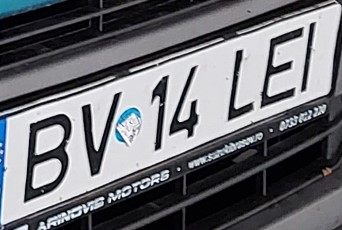
\includegraphics[width=0.4\textwidth]{images/color_roi.jpg}
    \caption{Segmentarea din imaginea de input}
\end{figure}
\FloatBarrier

Acum că regiunea de interes (ROI) pare să aibă dimensiuni similare cu un număr de înmatriculare, putem aplica diferiți algoritmi pentru a detecta contururile, care vor fi folosiți în pașii următori ai programului. Începem prin adăugarea unui padding la regiunea noastră de interes pentru a asigura continuitatea contururilor, evitând astfel întreruperi cauzate de dimensiunile măștilor utilizate pentru detectarea marginilor. Padding-ul este important pentru a ne asigura că niciun pixel relevant nu este omis în zonele limită.

\begin{figure}[htbp]
    \centering
    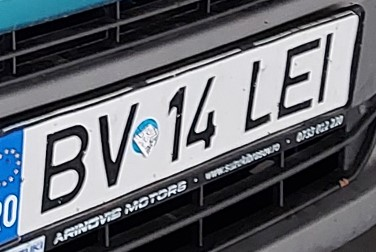
\includegraphics[width=0.4\textwidth]{images/padded_roi.jpg}
    \caption{Imaginea segmentată cu padding adăugat}
\end{figure}
\FloatBarrier

După aceasta, convertim segmentarea în format grayscale, deoarece algoritmii de detectare a marginilor necesită imagini în tonuri de gri.

\begin{figure}[htbp]
    \centering
    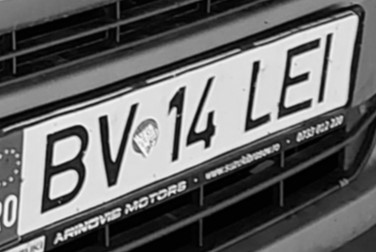
\includegraphics[width=0.4\textwidth]{images/gray_roi.jpg}
    \caption{Imaginea segmentată in format grayscale}
\end{figure}
\FloatBarrier

Primul pas este aplicarea filtrului Sobel, care detectează marginile bazându-se pe derivata imaginii. Pentru a obține o binarizare clară, aplicăm un filtru de binarizare Triangular Thresholding pentru a păstra doar pixelii relevanți detectați de Sobel, care sunt cu adevărat contururi.

\begin{figure}[htbp]
    \centering
    \begin{minipage}{0.4\textwidth}
        \centering
        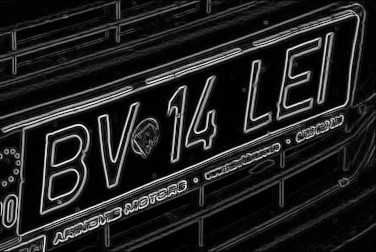
\includegraphics[width=1\textwidth]{images/sobel.jpg}
        \caption{Filtru Sobel}
    \end{minipage}
    \hspace{0.05\textwidth}
    \begin{minipage}{0.4\textwidth}
        \centering
        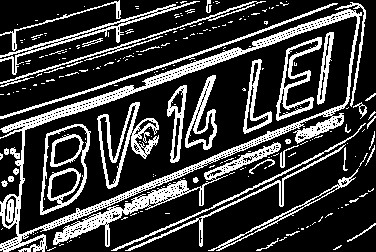
\includegraphics[width=1\textwidth]{images/binary_sobel.jpg}
        \caption{Filtru Sobel binarizat cu metoda Triangle Thresholding}
    \end{minipage}
\end{figure}
\FloatBarrier

Pentru a ne asigura că am captat toți pixelii relevanți din imagine, aplicăm și un filtru de obținere a gradientului morfologic tot pe regiunea în format grayscale, urmat de încă un filtru de binarizare Triangular Thresholding. Astfel, avem două imagini binare: una cu rezultatele filtrului Sobel și alta cu gradientul morfologic.

\begin{figure}[htbp]
    \centering
    \begin{minipage}{0.4\textwidth}
        \centering
        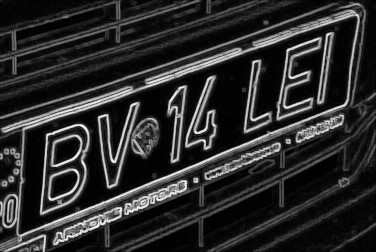
\includegraphics[width=1\textwidth]{images/gradient.jpg}
        \caption{Gradienții morfologici}
    \end{minipage}
    \hspace{0.05\textwidth}
    \begin{minipage}{0.4\textwidth}
        \centering
        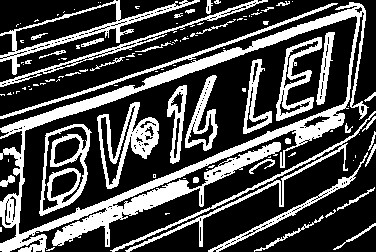
\includegraphics[width=1\textwidth]{images/binary_gradient.jpg}
        \caption{Gradienții morfologici binarizati}
    \end{minipage}
\end{figure}
\FloatBarrier

Următorul pas este combinarea acestor două imagini binare, păstrând în imaginea cu gradienții morfologici doar acei pixeli care apar în cel puțin una dintre imaginile binare.

\begin{figure}[htbp]
    \centering
    \begin{minipage}{0.4\textwidth}
        \centering
        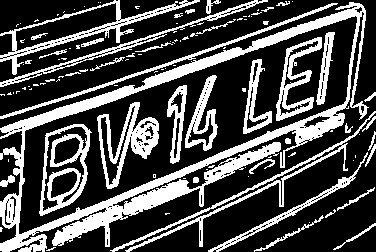
\includegraphics[width=1\textwidth]{images/or_binary.jpg}
        \caption{Reuniunea celor doua imagini binare (masca)}
    \end{minipage}
    \hspace{0.05\textwidth}
    \begin{minipage}{0.4\textwidth}
        \centering
        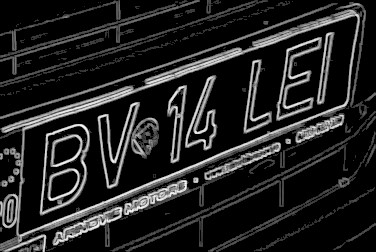
\includegraphics[width=1\textwidth]{images/or_gradient.jpg}
        \caption{Gradienții morfologici dupa mască}
    \end{minipage}
\end{figure}
\FloatBarrier

Acum, că avem doar pixelii care ar putea aparține unor contururi, aplicăm un filtru de subțiere Non-Maximum Suppression pentru a obține margini de un pixel grosime, astfel încât contururile să fie clare și precise.

\begin{figure}[htbp]
    \centering
    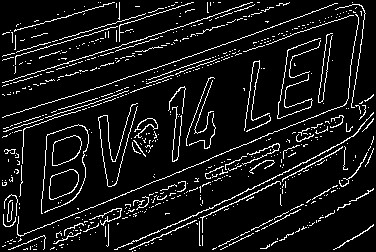
\includegraphics[width=0.4\textwidth]{images/non_maximum_suppression.jpg}
    \caption{Edge map de un pixel grosime}
\end{figure}
\FloatBarrier

În următorul pas, revenim la regiunea de interes în formatul grayscale și aplicăm un filtru de binarizare automatizat, cum ar fi Triangle Thresholding sau Otsu. Segmentarea este un dreptunghi în care ar trebui să fie inclus numărul de înmatriculare (dacă este regiunea corectă), dar în acesta pot exista și alte elemente din imaginea inițială care nu ne interesează.

\begin{figure}[htbp]
    \centering
    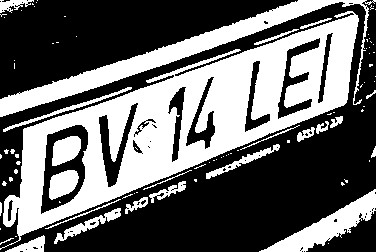
\includegraphics[width=0.4\textwidth]{images/before_roi.jpg}
    \caption{Imaginea segmentată cu filtru binar}
\end{figure}
\FloatBarrier

După aplicarea filtrului de binarizare, în imagine ar trebui observat un chenar alb care conține literele și cifrele numărului de înmatriculare și care ar trebui să fie separat de restul imaginii. Acum putem căuta din nou componentele conexe și păstra strict pe cea de dimensiunea cea mai mare, care ar trebui să fie chenarul alb. Însă pot apărea situații în care această binarizare este eronată și chenarul alb este conectat cu alte zone formate din pixeli albi.

Pentru a corecta acest lucru, folosim edge map-ul obținut anterior. Știm că în edge map contururile sunt reprezentate ca pixeli de valoare 255, deci putem verifica că pixelii albi (255) din edge map sunt negri (0) în regiunea binarizată. Acest lucru asigură că pixelii contururilor rămân separați și nu conectează eronat zonele între ele.

\begin{figure}[htbp]
    \centering
    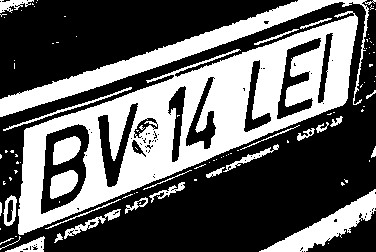
\includegraphics[width=0.4\textwidth]{images/after_roi.jpg}
    \caption{Corecția imaginii segmentate}
\end{figure}
\FloatBarrier

Pentru a fi complet siguri că nu există legături incorecte, putem aplica o operație morfologică de tip Opening. Această operație separă obiectele legate incorect prin linii fine.

După operația de Opening, este posibil să apară noi componente conexe, deci aplicăm din nou căutarea componentelor conexe și păstrăm doar componenta de dimensiunea cea mai mare. Aceasta ar trebui să fie chenarul alb care conține numărul de înmatriculare.

\begin{figure}[htbp]
    \centering
    
\includegraphics[width=0.4\textwidth]{images/roi.jpg}
    \caption{Regiunea textului}
\end{figure}
\FloatBarrier

Pentru a reduce numărul de segmente și pentru a ne apropia de regiunea care conține numărul de înmatriculare, putem adăuga o nouă condiție pentru imaginea segmentată, care ar trebui să conțină numai zona textului numărului de înmatriculare. Această condiție stabilește că înălțimea zonei respective ar trebui să fie aproape egală cu întreaga înălțime a imaginii de segmentare. Prin urmare, putem compara înălțimea acestei zone cu un procentaj, să zicem 80\%, din înălțimea regiunii de interes pentru a valida corectitudinea segmentării.
\[
    width > ROI.width \times percent; \, percent \in [0, 1]
\]

În pasul de rectificare, trebuie să obținem 4 coordonate pe baza cărora se va face rectificarea, aceste 4 coordonate fiind chiar colțurile chenarului alb în care se află numărul de înmatriculare. Pentru început, scădem din imaginea sursă imaginea sursă erodată pentru a obține exact conturul chenarului alb. Pe imaginea rezultată putem aplica algoritmul Hough, care ne va returna liniile din imagine, din intersectarea cărora putem obține coordonatele colțurilor.

\begin{figure}[htbp]
    \centering
    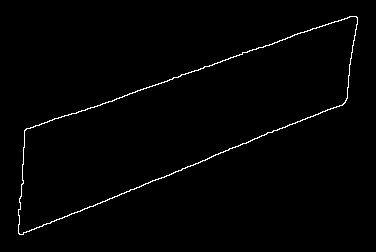
\includegraphics[width=0.4\textwidth]{images/edges.jpg}
    \caption{Conturul regiunii}
\end{figure}
\FloatBarrier

Pentru a face acest lucru, primul pas este să stabilim parametrii funcției Hough. Doi parametri importanți din funcția Hough sunt lungimea minimă admisă pentru o linie ca aceasta să fie adăugată ca rezultat și distanța maximă dintre două linii ca acestea să fie considerate de fapt aceeași linie, dar cu o întrerupere eronată între ele, și astfel în vectorul rezultat, în loc de două linii, să fie adăugată una singură formată din aceste două. Valorile acestor doi parametri sunt obținute în mod automatizat pe baza bounding box-ului rotit.

\begin{figure}[htbp]
    \centering
    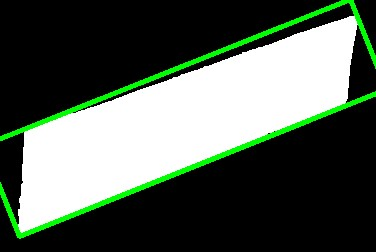
\includegraphics[width=0.4\textwidth]{images/rotated_rect.jpg}
    \caption{Bounding box-ul rotit al regiunii}
\end{figure}
\FloatBarrier

Având acest bounding box în care componenta conexă este încadrată exact, putem estima dimensiunile acesteia, deci și dimensiunile liniilor Hough. Astfel, pentru lungimea minimă a liniilor și distanța maximă dintre acestea, vom considera anumite procente din înălțimea bounding box-ului. Totuși, aceste procente pot fi destul de mici, de exemplu, 30\% pentru lungimea minimă a liniilor și 15\% pentru distanța maximă dintre acestea.

Această abordare este necesară deoarece, cu cât unghiul de fotografiere este mai inclinat, cu atât și numărul de înmatriculare va fi mai înclinat în imagine. În astfel de cazuri, algoritmul Hough, în loc să detecteze puține linii de dimensiuni mari, detectează multe linii de dimensiuni mici. Astfel, dacă stabilim valori mari parametrilor funcției, multe linii nu vor fi luate în calcul când numărul de înmatriculare este mai inclinat. Chiar și așa, dacă în continuare nu am obținut toate liniile de care aveam nevoie, putem decrementa treptat lungimea minimă a acestora, pentru a obține în final mai multe linii.

\begin{figure}[htbp]
    \centering
    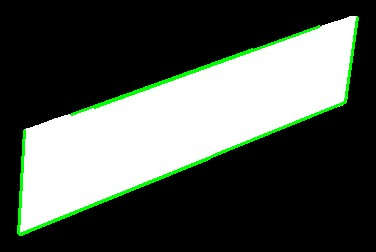
\includegraphics[width=0.4\textwidth]{images/lines.jpg}
    \caption{Liniile Hough}
\end{figure}
\FloatBarrier

Liniile de care avem nevoie sunt câte una din fiecare parte a chenarului alb, mai exact partea de sus, jos, stânga, dreapta, pentru că mai apoi să le putem găsi punctele de intersectie. Însă, algoritmul Hough nu ne oferă și informația de care parte aparține fiecare linie, așa că următoarea etapă este o sortare. Pentru început, vom sorta liniile ca fiind verticale sau orizontale. Putem obține această informație în funcție de panta fiecărei drepte:
\[
    slope = \frac{y_2 - y_1}{x_2 - x_1}
\]

Unghiul de înclinare se calculează apoi astfel:
\[
    angle = \lvert \arctan(slope) \times \frac{180}{\pi} \rvert
\]

Deci, dacă unghiul este aproape de 0 grade, linia este considerată orizontală, iar dacă este aproape de 90 de grade, linia este considerată verticală. Trebuie să ținem cont și de cazurile în care panta este complet verticală, pentru a evita împărțirea la zero.

\begin{figure}[htbp]
    \centering
    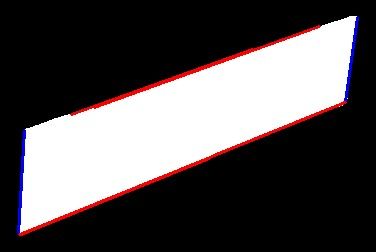
\includegraphics[width=0.4\textwidth]{images/horizontal_vertical_lines.jpg}
    \caption{Separarea liniilor verticale și orizontale}
\end{figure}
\FloatBarrier

După sortarea liniilor în verticale și orizontale, putem identifica liniile de care avem nevoie pentru fiecare parte a chenarului alb: partea de sus, jos, stânga, dreapta. Pentru a face acest lucru, luăm ca referință o linie verticală și una orizontală prin centrul imaginii, față de care se compară și se clasifică fiecare linie detectată de algoritmul Hough.

\begin{figure}[htbp]
    \centering
    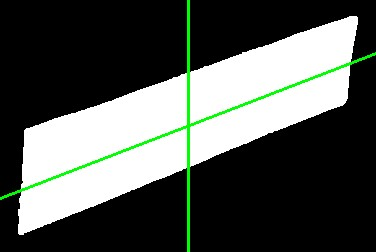
\includegraphics[width=0.4\textwidth]{images/reference_lines.jpg}
    \caption{Liniile de comparație}
\end{figure}
\FloatBarrier

În trasarea celor două linii de referință, vom ține cont și de pante, cel puțin în cazul celei orizontale, deoarece numărul de înmatriculare poate fi inclinat la un unghi atât de mare încât unele linii să fie clasificate eronat. În cazul în care numărul de înmatriculare este inclinat la un anumit unghi, și liniile trasate prin centrul imaginii trebuie să fie inclinate la unghiul respectiv pentru a se face clasificarea într-un mod corect.

După ce avem vectorii cu liniile orizontale și verticale, putem să-i parcurgem și să comparăm fiecare linie cu liniile de referință pentru a determina orientarea lor. Linia verticală de referință este utilizată pentru a compara liniile verticale, iar linia orizontală de referință pentru cele orizontale.

Pentru a face această comparație, putem folosi formula distanței dintre două drepte:
\[
    distance = (x - x_1) \cdot (y_2 - y_1) - (y - y_1) \cdot (x_2 - x_1)
\]

Semnul distanței ajută să separăm liniile detectate. Cele de deasupra liniei de referință vor avea distanțe pozitive, iar cele de dedesubt vor avea distanțe negative. La fel, liniile din dreapta vor avea distanțe pozitive față de linia de referință verticală, iar cele din stânga vor avea distanțe negative.

\begin{figure}[htbp]
    \centering
    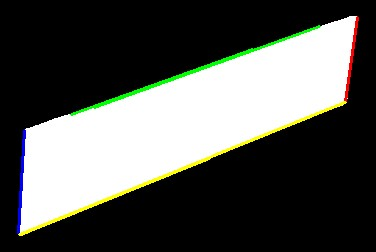
\includegraphics[width=0.4\textwidth]{images/multiple_lines.jpg}
    \caption{Clasificarea Liniile Hough}
\end{figure}
\FloatBarrier

Ideal, rezultatul ar trebui să fie compus din patru linii, câte una pentru fiecare parte a chenarului alb. Cu toate acestea, din cauza erorilor de detectare sau a înclinațiilor, pot apărea mai multe segmente în loc de o singură linie. Dacă avem mai multe segmente, putem căuta capetele cele mai îndepărtate în funcție de orientare pentru a le lega între ele și a obține o singură linie pentru fiecare parte.

\begin{figure}[htbp]
    \centering
    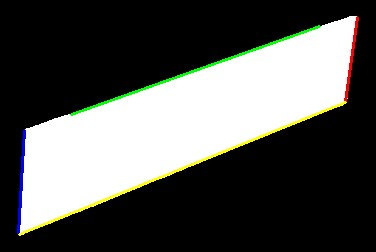
\includegraphics[width=0.4\textwidth]{images/sorted_lines.jpg}
    \caption{Cele 4 linii rezultate}
\end{figure}
\FloatBarrier

Acesta este și momentul în care verificăm dacă trebuie să aplicăm din nou algoritmul Hough cu parametrii ajustați sau dacă am găsit toate liniile necesare. Dacă avem cele patru linii căutate, pasul următor este să calculăm punctele de intersecție între ele pentru a obține coordonatele colțurilor chenarului alb. Ordinea este următoarea:
\begin{itemize}
    \item Punctul din stânga sus se obține prin intersectarea liniei din stânga cu cea de sus.
    \item Punctul din dreapta sus se obține prin intersectarea liniei din dreapta cu cea de sus.
    \item Punctul din dreapta jos se obține prin intersectarea liniei din dreapta cu cea de jos.
    \item Punctul din stânga jos se obține prin intersectarea liniei din stânga cu cea de jos.
\end{itemize}

\begin{figure}[htbp]
    \centering
    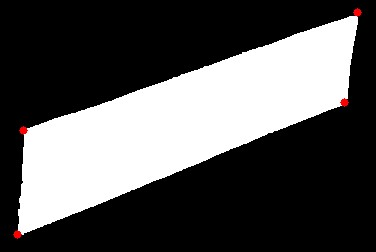
\includegraphics[width=0.4\textwidth]{images/points.jpg}
    \caption{Punctele de rectificare}
\end{figure}
\FloatBarrier

O problemă des întâlnită cu liniile detectate este că punctele de intersecție pot fi în afara imaginii, ceea ce necesită un padding suficient de mare pentru a cuprinde toate cele patru puncte de intersecție. Pentru a rezolva această situație, trebuie să căutăm coordonatele cele mai mici și cele mai mari pentru X și Y dintre punctele calculate anterior:
\[
    \begin{aligned}
        minX & = ROI.width, \, minY = ROI.height, \ maxX = 0, \, maxY = 0,
    \end{aligned}
\]
Pentru fiecare punct (\(x, y\)):
\[
    \begin{aligned}
        minX & = \min(minX, x); \\
        minY & = \min(minY, y); \\
        maxX & = \max(maxX, x); \\
        maxY & = \max(maxY, y).
    \end{aligned}
\]

După ce avem aceste valori, putem calcula dimensiunea padding-ului necesar pentru fiecare parte a imaginii. Dacă punctele de intersecție sunt în afara imaginii, vom ajusta padding-ul pentru a le include:
\[
    \begin{aligned}
        paddingRight  & = \max(0, maxX - (src.cols - 1)), \\
        paddingBottom & = \max(0, maxY - (src.rows - 1)), \\
        paddingLeft   & = \max(0, -minX),                 \\
        paddingTop    & = \max(0, -minY).
    \end{aligned}
\]

Această abordare ne permite să ajustăm imaginea astfel încât toate punctele de intersecție să fie incluse în limitele acesteia, inclusiv punctele care au coordonate mai mari decât dimensiunile imaginii inițiale. Însă, dacă există și puncte cu coordonate negative pentru care a fost adăugat padding în partea de sus a imaginii sau în partea din stânga, suntem nevoiți să ajustăm toate punctele de intersecție cu valoarea padding-ului adăugat pentru a reflecta noua poziție în cadrul imaginii extinse:

Pentru fiecare punct (\(x, y\)):
\[
    \begin{aligned}
        x = paddingLeft + x, \\
        y = paddingTop + y.
    \end{aligned}
\]

Acum că avem cele patru coordonate ale colțurilor chenarului alb și ne-am asigurat că sunt în interiorul imaginii, putem trece la pasul de rectificare. Rectificarea presupune transformarea geometrică a regiunii de interes pentru a alinia numărul de înmatriculare într-o poziție corectă, obținând astfel o imagine rectificată.

Pentru a începe procesul de rectificare, calculăm dimensiunile imaginii rezultate. Pentru a determina înălțimea corectă a numărului de înmatriculare, scădem coordonata Y a punctului din stânga sus din coordonata Y a punctului din stânga jos:
\[
    height = DownLeft.y - UpLeft.y
\]

Pentru a obține lățimea, folosim raportul cunoscut pentru numărul de înmatriculare, unde lățimea este de 4.3 ori mai mare decât înălțimea:
\[
    width = 4.3 \times height
\]

Cu aceste dimensiuni calculate, putem stabili punctele corespunzătoare pentru fiecare colț al chenarului alb în imaginea destinată. Ordinea punctelor pentru colțurile chenarului alb este: stânga sus, dreapta sus, dreapta jos, stânga jos. Pentru imaginea rectificată, punctele corespondente vor fi:
\begin{itemize}
    \item (0, 0) pentru stânga sus,
    \item (width - 1, 0) pentru dreapta sus,
    \item (width - 1, height - 1) pentru dreapta jos,
    \item (0, height - 1) pentru stânga jos.
\end{itemize}

\begin{figure}[htbp]
    \centering
    
\includegraphics[width=0.4\textwidth]{images/points_on_black.jpg}
    \caption{Punctele de rectificare in imaginea destinație}
\end{figure}
\FloatBarrier

Cu aceste puncte corespondente, putem calcula matricea de transformare utilizând funcția de transformare geometrică. Aplicând această transformare pe imaginea segmentată în formatul grayscale, obținem în final numărul de înmatriculare într-o formă rectificată.

\begin{figure}[htbp]
    \centering
    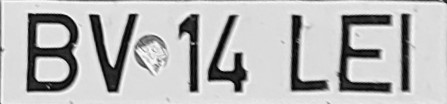
\includegraphics[width=0.4\textwidth]{images/transformed.jpg}
    \caption{Imaginea rectificată}
\end{figure}
\FloatBarrier

Imaginea rezultată ar trebui să conțină literele și cifrele numărului de înmatriculare pe fundal alb. Însă, există și situații în care rectificarea nu este tocmai ideală, iar astfel pot apărea diverse probleme: anumite caractere nu sunt în totalitate incadrate în imagine, iar astfel, spre exemplu, un caracter este ușor tăiat într-o parte anume, sau, în cazul opus, zona rectificată este ușor mai mare și astfel se obțin detalii în plus la extremitățile imaginii, detalii ce nu sunt necesare.

Ca o primă soluție este decuparea de pe fiecare parte a imaginii a câte o linie sau a câte o coloană, ca mai apoi să se adauge un padding alb în locul liniilor și coloanelor decupate. Decupând o mică parte din imagine, se reduce din posibila zonă care este în plus. De asemenea, padding-ul alb de jur împrejurul imaginii asigură că nu va exista un contur discontinuu al chenarului alb, cum s-ar întâmpla în cazul în care o literă nu este întru totul încadrată în imagine și întrerupe conturul dreptunghiular al chenarului.

\begin{figure}[htbp]
    \centering
    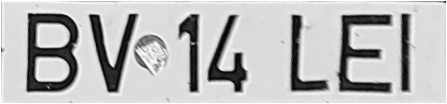
\includegraphics[width=0.4\textwidth]{images/boardered.jpg}
    \caption{Imaginea rectificată cu padding adăugat}
\end{figure}
\FloatBarrier

Următorul pas este aplicarea unui filtru Binary Thresholding pe imaginea rectificată. Acest lucru va crea o imagine binarizată în care literele și cifrele numărului de înmatriculare vor fi separate de fundal. Însă, se aplică și un filtru de inversare a culorilor deoarece caracterele sunt de culoare neagră pe un fundal alb, pe când acestea ar trebui să fie albe pe un fundal negru.

\begin{figure}[htbp]
    \centering
    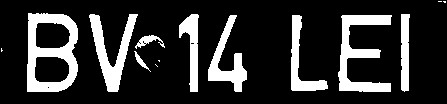
\includegraphics[width=0.4\textwidth]{images/text.jpg}
    \caption{Imaginea rectificată cu filtru binar}
\end{figure}
\FloatBarrier

Caracterele numărului de înmatriculare pot fi considerate și componente conexe în imaginea binară. De asemenea, știm că numerele de înmatriculare în formatul din România au între 6 și 8 caractere, deci tot atâtea componente conexe trebuie să existe în imaginea binară. Însă, nu este întotdeauna așa, căci uneori numărul de înmatriculare poate avea diferite însemnări pe care le vom considera artefacte și pe care dorim să le eliminăm.

O primă etapă este detectarea tuturor componentelor conexe din imagine și ordonarea acestora după aria lor. Cele mai mari componente conexe tind să fie caracterele numărului de înmatriculare. După ordonare, păstrăm primele opt componente, deoarece, așa cum am stabilit, un număr de înmatriculare nu are mai mult de opt caractere.

\begin{figure}[htbp]
    \centering
    
\includegraphics[width=0.4\textwidth]{images/before_denoise.jpg}
    \caption{Primele 8 componente conexe}
\end{figure}
\FloatBarrier

Cu toate acestea, tot este posibil ca una sau două componente conexe din imagine să fie de fapt zgomot. Pentru a detecta și elimina posibilul zgomot, putem folosi înălțimea ca un factor comun între caractere. Calculăm înălțimea mediană a componentelor conexe și o folosim ca referință pentru a compara înălțimea fiecărei componente cu cea mediană:
\[
    \left| median - height \right| > median \times percent; \, percent \in [0, 1]
\]

Dacă diferența dintre înălțimea componentei conexe curente și cea mediană este mai mare decât un anumit procent din înălțimea mediană, de exemplu 20\%, putem considera acea componentă ca fiind zgomot și se elimină. Prin aplicarea acestui filtru bazat pe înălțime, ne putem asigura că imaginea finală conține doar componentele conexe care corespund literelor și cifrelor numărului de înmatriculare.

\begin{figure}[htbp]
    \centering
    
\includegraphics[width=0.4\textwidth]{images/after_denoise.jpg}
    \caption{Eliminarea componentelor conexe eronate}
\end{figure}
\FloatBarrier

De asemenea, ca la un pas anterior, pentru a fi complet siguri că nu există legături incorecte între componentele conexe, putem aplica și o operație morfologică de tip Opening. Această operație separă obiectele legate incorect prin linii fine.

După operația de Opening, este posibil să apară noi componente conexe, motiv pentru care se aplică din nou funcția descrisă anterior și astfel se elimină noile componente conexe, care nu sunt caractere, rezultate din urma operației morfologice.

În urma aplicării tuturor tehnicilor de procesare a imaginilor, am obținut o imagine în care textul numărului de înmatriculare arată ca și cum ar fi fost tastat manual într-un fișier. Aceasta este o imagine potrivită pentru modelul de recunoaștere a caracterelor Tesseract OCR. Totuși, pentru a obține rezultate mai bune, este util să furnizăm modelului AI fiecare caracter separat, pe rând.

Pentru a realiza acest lucru, aplicăm pe imaginea binară rectificată funcția implementată într-un pas anterior ce detectează componentele conexe, pentru a obține bounding box-urile tuturor caracterelor. Rezultatul este din nou un vector ce conține coordonatele colțului din stânga sus ale fiecărui bounding box, precum și înălțimea și lățimea fiecărei componente. Este important să cunoaștem ordinea corectă a caracterelor în imagine pentru a putea reconstrui textul numărului de înmatriculare din caracterele recunoscute.

\begin{figure}[htbp]
    \centering
    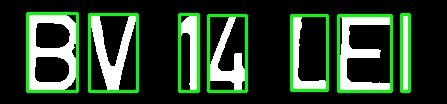
\includegraphics[width=0.4\textwidth]{images/chars.jpg}
    \caption{Bounding box-urile caracterelor}
\end{figure}
\FloatBarrier

Cu toate acestea, ordinea în care componentele conexe sunt stocate în vector poate să nu coincidă cu ordinea reală a caracterelor în imagine. Pentru a remedia acest lucru, sortăm vectorul în ordine crescătoare după coordonata X a fiecărui bounding box. Astfel, obținem o ordine a componentelor conexe care corespunde ordinii reale a caracterelor din imagine.

Știm că numerele de înmatriculare care respectă formatul din România conțin una sau două litere, urmate de două sau trei cifre, și încheiate cu alte trei litere. Această structură ne poate ajuta să îmbunătățim recunoașterea caracterelor. În următoarea etapă, vom partitiona caracterele numărului de înmatriculare în trei regiuni.

Deși știm numărul total de caractere din imagine, primele două regiuni ale numărului de înmatriculare pot avea un număr variabil de caractere, ceea ce înseamnă că nu știm exact unde se termină prima regiune și începe a doua. Pentru a determina acest lucru, trebuie să calculăm distanțele dintre colțurile bounding box-urilor vecine și să identificăm distanța cea mai mare, deoarece aceasta va fi între prima și a doua regiune a numărului de înmatriculare.

Odată ce am identificat cea mai mare distanță între componentele conexe, putem partitiona caracterele în funcție de regiuni:
\begin{itemize}
    \item Prima regiune: cuprinde toate componentele conexe de la început până la cea dinaintea distanței calculate.
    \item A doua regiune: începe de la componenta conexă imediat după distanța cea mai mare și se întinde până la componenta conexă dinaintea ultimelor trei.
    \item A treia regiune: include ultimele trei componente conexe, începând de la antepenultima și terminând cu ultima.
\end{itemize}

Intr-un final, se memoreaza indexul de început pentru fiecare regiune.

\begin{figure}[htbp]
    \centering
    
\includegraphics[width=0.4\textwidth]{images/partitioned.jpg}
    \caption{Clasificarea caracterelor}
\end{figure}
\FloatBarrier

Tesseract OCR poate primi ca input imaginea binară cu textul complet și apoi i se pot specifica zonele pentru recunoașterea caracterelor, bazându-ne pe bounding box-uri. Cu toate acestea, bounding box-urile nu includ spațiu pentru padding, ceea ce este esențial pentru model AI. De aceea, vom segmenta fiecare caracter din imagine conform bounding box-urilor și îi vom adăuga padding.

Numărul de linii și coloane pentru padding poate fi calculat automat, folosind un procent din dimensiunile bounding box-ului. Vom considera un procent semnificativ, cum ar fi 60\%. Prin înmulțirea acestui procent cu înălțimea și lățimea bounding box-ului, putem determina numărul de linii și coloane care trebuie adăugate în jurul imaginii segmentate pentru a oferi suficient spațiu:

\[
    \begin{aligned}
        paddingX & = BBox.width \times percent  \\
        paddingY & = BBox.height \times percent
    \end{aligned}
\]

Însă, înainte de a adăuga padding fiecărui caracter, este necesar să actualizăm informațiile legate de bounding box. Dimensiunile padding-ului trebuie adăugate la dimensiunile inițiale ale bounding box-ului, de două ori, deoarece padding-ul este aplicat pe ambele părți ale imaginii, atât pe axa X, cât și pe axa Y:

\[
    \begin{aligned}
        BBox.width  & = BBox.width + paddingX \times 2,  \\
        BBox.height & = BBox.height + paddingY \times 2,
    \end{aligned}
\]

Revenim la bounding box-urile inițiale, pe baza cărora vom realiza segmentările în imaginea binară pentru a extrage fiecare caracter. Din bounding box-uri cu padding-ul asociat, putem extrage valoarea specifică a padding-ului pentru fiecare caracter și apoi o putem adăuga la imaginea segmentată.

După ce toate caracterele segmentate sunt obținute, fiecare având padding-ul adăugat, următorul pas este concatenarea lor într-un singur șir, recreând astfel textul inițial cu această nouă distanțare.

Va trebui să generăm, de asemenea, o imagine complet neagră de dimensiuni suficient de mari pentru a cuprinde toate caracterele, împreună cu padding-ul lor. În primul rând, vom determina înălțimea acesteia, care va fi echivalentă cu înălțimea celui mai înalt bounding box. Lățimea va fi calculată ca suma tuturor lățimilor bounding box-urilor.

Anterior, am ajustat dimensiunile bounding box-urilor pentru a se potrivi cu padding-ul, însă acum trebuie să modificăm și colțurile acestora. Coordonata X a fiecărui bounding box poate fi calculată ca suma lățimilor bounding box-urilor anterioare acestuia, iar coordonata Y poate fi calculată ca diferența dintre înălțimea imaginii și înălțimea bounding box-ului, împărțită la 2, pentru a centra caracterul pe axa Y:
\[
    \begin{aligned}
        width & = 0,
    \end{aligned}
\]
Pentru fiecare bounding box:
\[
    \begin{aligned}
        y     & = \frac{height - BBox.height}{2}, \\
        x     & = width,                          \\
        width & = width + BBox.width.
    \end{aligned}
\]

Din acest punct, revenim la segmentele realizate anterior pentru fiecare caracter și le inserăm, pe rând, în imaginea complet neagră generată anterior, conform noilor bounding box-uri.

\begin{figure}[htbp]
    \centering
    
\includegraphics[width=0.4\textwidth]{images/spaced.jpg}
    \caption{Spațierea caracterelor}
\end{figure}
\FloatBarrier

Acum, cunoscând atât bounding box-urile cu padding, cât și cele fără padding, putem folosi indicii obținuți anterior pentru a separa aceste bounding box-uri în funcție de regiunile de care aparțin.

Pe baza acestor indici, se pot impune condiții suplimentare pentru a ne asigura că segmentarea imaginii originale conține într-adevăr numărul de înmatriculare. Se verifică dacă al doilea indice este egal cu 2 sau 3, deoarece s-a stabilit că prima regiune poate avea maximum două caractere. De asemenea, se verifică dacă intervalul dintre al doilea și al treilea indice conține exact două sau trei caractere.

Următorul pas implică utilizarea modelului AI Tesseract OCR pentru recunoașterea textului în imagine. Se creează o instanță de tip tesseract::TessBaseAPI și se dezactivează toate dicționarele implicite, deoarece acestea nu sunt necesare în acest context. Se setează și un whitelist care indică dacă modelul trebuie să caute litere sau cifre, în funcție de regiunea în care se află caracterul dintre cele trei regiuni obținute anterior.

Modelului i se oferă ca input imaginea binară cu caracterele distanțate și se parcurg, pe rând, fiecare dintre bounding box-uri pentru a specifica zonele în care să se recunoască textul.

\begin{figure}[htbp]
    \centering
    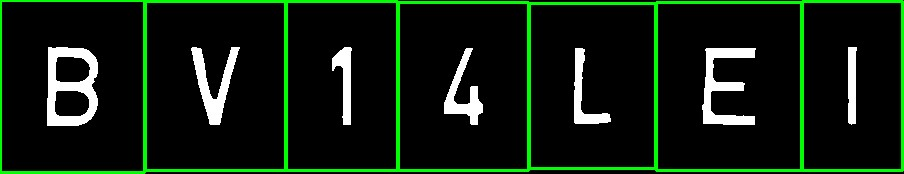
\includegraphics[width=0.4\textwidth]{images/input_ocr.jpg}
    \caption{Bounding box-urile caracterelor cu padding adăugat (input-uri OCR) }
\end{figure}
\FloatBarrier

Dacă în segmentul de imagine nu a fost recunoscut niciun caracter sau au fost recunoscute mai multe, se decrementează dimensiunea bounding box-ului și se încearcă din nou recunoașterea, sperând că de această dată să fie identificat caracterul corect. Decrementarea continuă până când bounding box-ul revine la dimensiunile inițiale, încadrând caracterul cu precizie minimă:
\[
    \begin{aligned}
        x      & = x - 1,      \\
        y      & = y - 1,      \\
        width  & = width - 2,  \\
        height & = height - 2.
    \end{aligned}
\]

\begin{figure}[htbp]
    \centering
    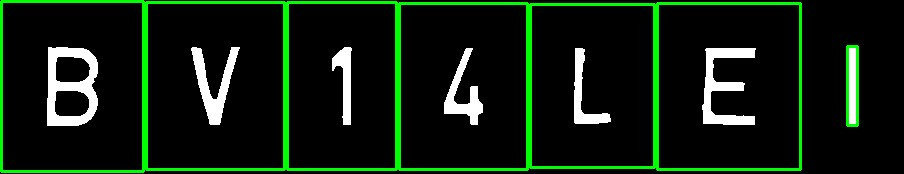
\includegraphics[width=0.4\textwidth]{images/output_ocr.jpg}
    \caption{Decrementarea bounding box-urilor până la recunoaștere corectă a caracterelor}
\end{figure}
\FloatBarrier

Dacă totuși bounding box-ul a revenit la dimensiunile inițiale și modelul AI nu a reușit să recunoască caracterul din imagine, este posibil ca problema să fie cauzată de litera "I". În anumite cazuri, Tesseract OCR nu recunoaște acest caracter, așa că se utilizează o tehnică de Template matching pentru a determina dacă respectivul caracter nerecunoscut este "I" sau nu.

\begin{figure}[htbp]
    \centering
    
\includegraphics[height=0.2\textwidth]{images/i.jpg}
    \caption{Segmentarea literei nerecunoscute}
\end{figure}
\FloatBarrier

În pasul de template matching, se încărca în program o imagine template pentru litera "I".

\begin{figure}[htbp]
    \centering
    
\includegraphics[height=0.2\textwidth]{images/template.jpg}
    \caption{Template-ul literei "I"}
\end{figure}
\FloatBarrier

Pentru început, redimensionăm această imagine template la dimensiunile caracterului segmentat. Vom calcula raportul de aspect pentru imaginea template și noua lățime pe care o va avea:

\[
    \begin{aligned}
        aspectRation   & = Template.width / Template.height, \\
        Template.width & = Sursa.height * aspectRadion.
    \end{aligned}
\]

Pe imaginea redimensionată, se aplică un filtru de tip "Binary Thresholding" pentru a obține regiunea exactă a literei.

\begin{figure}[htbp]
    \centering
    
\includegraphics[height=0.2\textwidth]{images/binary_template.jpg}
    \caption{Template-ul literei "i" cu filtru binar}
\end{figure}
\FloatBarrier

În acest moment, litera poate fi înconjurată neuniform de linii și coloane negre, motiv pentru care dorim să o extragem din imaginea inițială și să creăm o imagine în care litera să aibă un spațiu uniform pe toate laturile. Astfel, se caută contururile în imagine pentru a identifica conturul singurei regiuni albe existente, care reprezintă litera. Pe baza acestui contur, se extrage litera din imagine și se inserează într-o imagine complet neagră cu dimensiuni egale cu cele ale literei, dar cu un padding de o unitate pe toate laturile.

Deși template-ul a fost redimensionat la înălțimea segmentării, din cauza uniformizării padding-ului, este posibil ca dimensiunea să nu rămână cea stabilită inițial. Prin urmare, vom calcula diferența dintre aceste două înălțimi pentru a obține padding-ul suplimentar care trebuie adăugat la șablon în partea de sus și de jos. Această diferență se împarte la jumătate pentru a adăuga aceeași cantitate de padding pe fiecare parte a imaginii. De asemenea, se verifică dacă această diferență este pară, deoarece, în caz contrar, va trebui incrementat padding-ul pe una dintre părți:
\[
    \begin{aligned}
        firstPadding  & = \frac{Sursa.height - Template.height}{2},               \\
        secondPadding & = firstPadding,                                           \\
        secondPadding & = \text{secondPadding} + 1,                               \\
                      & \text{dacă } (Sursa.height - Template.height) \mod 2 = 1.
    \end{aligned}
\]

Pentru a stabili și lățimea imaginii template, se va adăuga un padding similar cu cel anterior, calculat pe baza diferenței dintre lățimea imaginii sursă și lățimea imaginii template. La fel ca înainte, diferența se împarte la jumătate pentru a determina padding-ul care trebuie adăugat de fiecare parte a șablonului și se verifică dacă diferența este pară, astfel încât padding-ul să fie distribuit uniform:
\[
    \begin{aligned}
        firstPadding  & = \frac{Sursa.width - Template.width}{2},               \\
        secondPadding & = firstPadding,                                         \\
        secondPadding & = \text{secondPadding} + 1,                             \\
                      & \text{dacă } (Sursa.width - Template.width) \mod 2 = 1.
    \end{aligned}
\]

Acum că cele două imagini sunt ajustate la aceeași dimensiune și cu litera "I" reprezentată central după adăugarea padding-ului, se realizează intersectarea celor două regiuni albe utilizând operația logică 'și'.

\begin{figure}[htbp]
    \centering
    
\includegraphics[height=0.2\textwidth]{images/intersection.jpg}
    \caption{Intersecția celor doua imagini}
\end{figure}
\FloatBarrier

Scorul Dice poate fi calculat pe baza acestei intersecții, indicând cât de mult se suprapun cele două regiuni. Dacă scorul obținut este semnificativ, de exemplu cel puțin 80\%, se poate concluziona că respectivul caracterul nerecunoscut este 'I'. În caz contrar, se consideră că segmentarea inițială nu reprezintă numărul de înmatriculare și se continuă cu următoarea iterație.

În ultima etapă, se compune textul numărului de înmatriculare folosind caracterele recunoscute, se calculează o medie a nivelului de încredere pe baza tuturor scorurilor de încredere obținute pentru fiecare caracter, se memorează data și ora curente, iar în imaginea sursă se desenează un chenar care încadrează numărul de înmatriculare, pe baza segmentării inițiale.

\begin{figure}[htbp]
    \centering
    
\includegraphics[width=0.4\textwidth]{images/output.jpg}
    \caption{Imaginea de output}
\end{figure}
\FloatBarrier

În situația în care nu a fost recunoscut textul integral al numărului de înmatriculare, acesta este catalogat drept "necunoscut".

Pentru toate componentele descrise anterior, s-au dezvoltat un set de teste în cadrul proiectului „Tests” pentru a asigura robustețea și fiabilitatea aplicației. Aceste teste sunt concepute pentru a evalua comportamentul fiecărei funcții în condiții diverse, cum ar fi procesarea imaginilor neinițializate sau cu un număr diferit de canale față de cel așteptat, și manipularea pixelilor de un tip de date diferit. Aceasta abordare ajută în identificarea punctelor slabe ale procesării și asigură că modulele pot gestiona orice tip de intrare în mod corect.

Pentru funcțiile matematice în special, s-au implementat teste pentru a preveni erori precum împărțirile la zero și alte situații excepționale care pot apărea în timpul execuției. Aceste teste sunt vitale pentru a evita crash-uri ale aplicației și pentru a asigura că output-ul matematic este întotdeauna valid și precis.

Ca rezultat al acestor teste, în codul fiecărei funcții s-au adăugat multiple condiții de verificare a datelor de intrare. Aceste verificări suplimentare asigură că, indiferent de variațiile datelor de intrare, funcțiile vor răspunde în mod adecvat, trecând testele și evitând posibilele erori care ar putea să compromită funcționalitatea aplicației.

\section{Pipeline pentru detectarea codurilor QR}

În continuare, dorim să analizăm pașii principali ai pipeline-ului de detecție a codurilor QR. Funcționalitățile sunt implementate în cadrul clasei \textit{QRCode}, care face parte din modulul dedicat procesării imaginilor. 

\begin{figure}[htbp]
    \centering
    
\includegraphics[width=0.85\textwidth]{images/qr_pipeline.png}
    \caption{Pașii esențiali în identificarea și rectificarea unui cod QR
}
\end{figure}
\FloatBarrier

Pentru o mai bună înțelegere, vom considera o imagine de intrare exemplu și vom descrie fiecare etapă a procesului.

Primul pas în cadrul pipeline-ului constă în redimensionarea imaginii de intrare. Această etapă are rolul de a normaliza dimensiunea imaginii, astfel încât procesările ulterioare să fie mai eficiente din punct de vedere computațional și mai stabile.

Funcția de redimensionare păstrează raportul de aspect al imaginii și limitează dimensiunea maximă a acesteia la o valoare prestabilită. În funcție de orientarea imaginii (portret, landscape sau pătrat), aceasta este scalată corespunzător:
\begin{itemize}
    \item dacă înălțimea este mai mare decât lățimea, imaginea este redimensionată astfel încât înălțimea să devină egală cu valoarea maximă;
    \item dacă lățimea este mai mare decât înălțimea, aceasta este scalată la dimensiunea maximă;
    \item dacă imaginea este pătrată, ambele dimensiuni sunt reduse uniform;
    \item în cazul în care imaginea este deja mai mică decât dimensiunea maximă, aceasta rămâne neschimbată.
\end{itemize}

\begin{figure}[htbp]
    \centering
    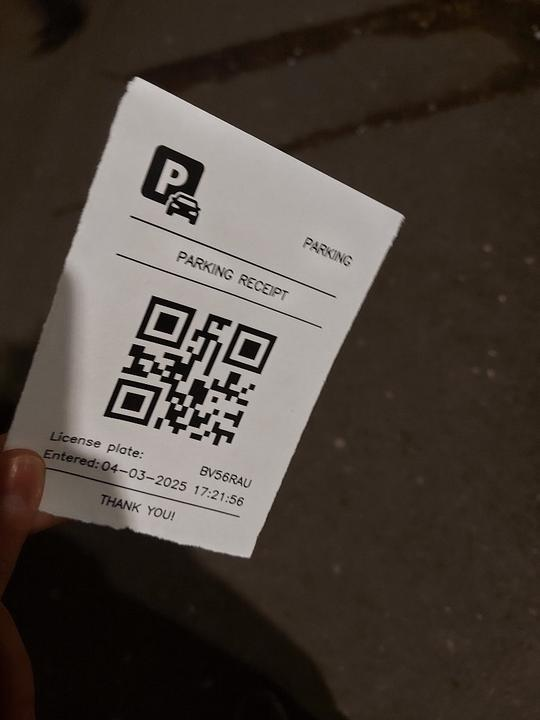
\includegraphics[width=0.25\textwidth]{images/qr1.jpg}
    \caption{Imaginea de input}
\end{figure}
\FloatBarrier

După redimensionarea imaginii, următorul pas constă în conversia acesteia în format grayscale. Această etapă este necesară deoarece algoritmii de detecție a marginilor operează pe imagini cu un singur canal.

\begin{figure}[htbp]
    \centering
    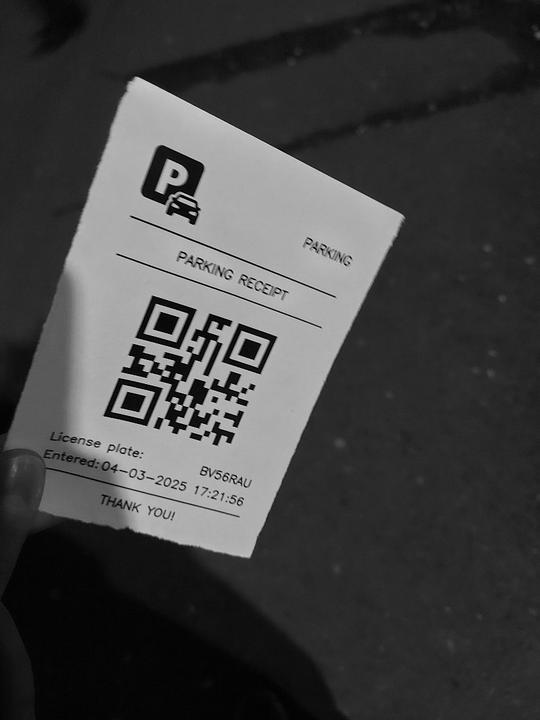
\includegraphics[width=0.25\textwidth]{images/qr2.jpg}
    \caption{Imaginea în format grayscale}
\end{figure}
\FloatBarrier

În continuare, se aplică operatorul Sobel pe cele două direcții ale imaginii, Ox și Oy. Pe baza acestor derivate se calculează magnitudinea gradientului, precum și direcția acestuia pentru fiecare pixel. Magnitudinea este normalizată în intervalul $[0, 255]$, astfel încât valorile obținute să poată fi procesate ulterior ca imagine grayscale.

Pentru a elimina variațiile nesemnificative și a păstra doar muchiile relevante, magnitudinea gradientului este binarizată folosind metoda Otsu. Masca binară rezultată este apoi aplicată peste magnitudinea normalizată, obținându-se o imagine în care sunt păstrate doar zonele cu tranziții puternice de intensitate.

\begin{figure}[htbp]
    \centering
    \begin{minipage}{0.25\textwidth}
        \centering
        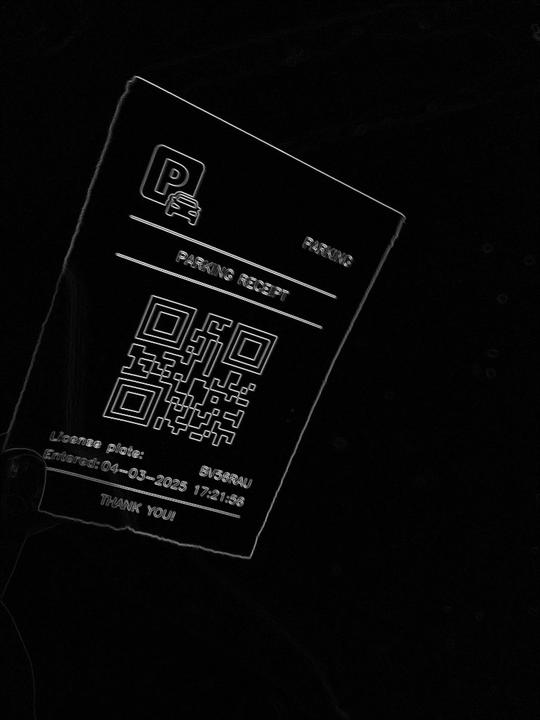
\includegraphics[width=1\textwidth]{images/qr3.jpg}
        \caption{Magnitudinea gradientului Sobel}
    \end{minipage}
    \hspace{0.04\textwidth}
    \begin{minipage}{0.25\textwidth}
        \centering
        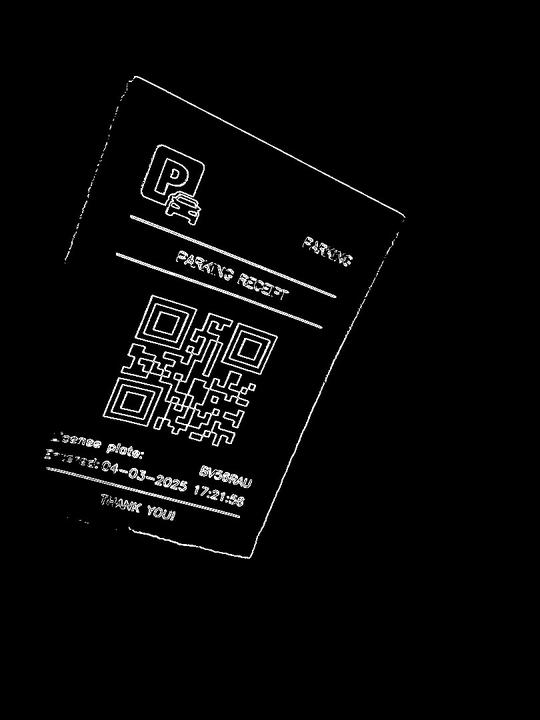
\includegraphics[width=1\textwidth]{images/qr4.jpg}
        \caption{Magnitudinea Sobel filtrată prin metoda Otsu}
    \end{minipage}
\end{figure}
\FloatBarrier

În continuare, se aplică etapa de \textit{Non-Maximum Suppression}. Aceasta folosește direcția gradientului pentru a compara fiecare pixel cu vecinii săi aflați pe aceeași direcție a muchiei. Dacă pixelul curent reprezintă un maxim local, acesta este păstrat; în caz contrar, este eliminat.

Rezultatul acestei etape este o hartă de margini subțiată, în care contururile au grosime de aproximativ un pixel. Acest lucru este important pentru detecția codurilor QR, deoarece acestea sunt formate din tranziții dese între zone albe și negre, iar o hartă de muchii clară facilitează identificarea regiunilor cu structură specifică unui cod QR.

\begin{figure}[htbp]
    \centering
    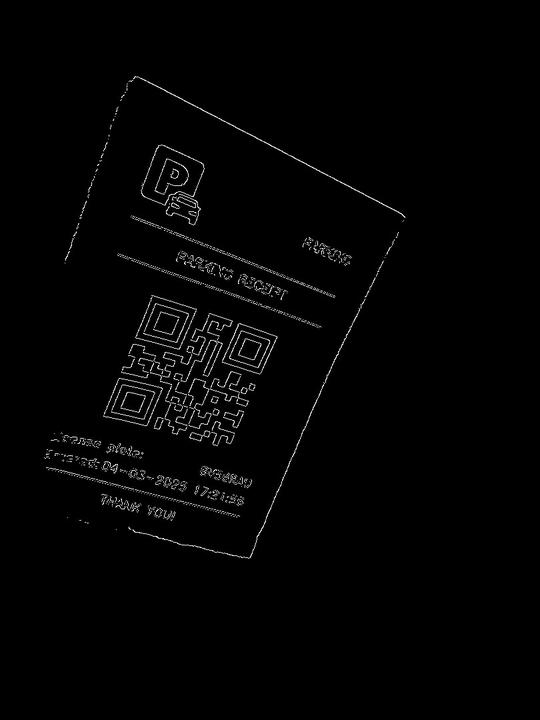
\includegraphics[width=0.25\textwidth]{images/qr5.jpg}
    \caption{Harta de margini obținută după Non-Maximum Suppression}
\end{figure}
\FloatBarrier

După obținerea hărții de margini, detecția se concentrează pe identificarea celor trei marcatori de poziționare ai codului QR, numiți în continuare ancore. Această abordare este apropiată de structura internă a unui cod QR, deoarece cei trei marcatori sunt formați din pătrate concentrice și pot fi detectați prin analiza contururilor și a ierarhiei acestora.

Pentru început, harta de margini este prelucrată printr-o operație morfologică de tip închidere, folosind un element de structură dreptunghiular de dimensiune $3 \times 3$. Această operație are rolul de a conecta mici întreruperi apărute în contururi după etapa de detecție a muchiilor și \textit{Non-Maximum Suppression} și pentru a stabiliza contururile care vor fi analizate ulterior.

\[
    edges_{closed} = \operatorname{Close}(edges, K_{3 \times 3})
\]

Pe imaginea rezultată sunt extrase contururile folosind o ierarhie de tip arbore. Această ierarhie este importantă deoarece marcatorii de poziționare ai codurilor QR conțin mai multe contururi imbricate. Astfel, nu se analizează doar forma unui contur izolat, ci și relația dintre acesta și contururile aflate în interiorul său.

Pentru fiecare contur de nivel superior, adică pentru fiecare contur care nu are părinte în ierarhie, se aplică mai întâi o filtrare geometrică. Contururile cu arie prea mică sunt eliminate, iar contururile rămase sunt aproximate poligonal folosind metoda \textit{Douglas-Peucker}. Un contur este considerat candidat pentru o ancoră QR doar dacă aproximația sa are patru vârfuri, deoarece marcatorii de poziționare au formă aproximativ pătrată.

\[
    area(contour) \geq 10
\]

\[
    \epsilon = 0.02 \cdot perimeter
\]

\[
    \left|\mathcal{P}_{\epsilon}(C)\right| = 4
\]

După această filtrare, pentru fiecare contur candidat este analizată structura sa internă. Pornind de la conturul curent, se caută recursiv cel mai mare copil din ierarhie, iar apoi cel mai mare copil al acestuia și așa mai departe. La fiecare pas se compară forma conturului curent cu forma copilului selectat. În acest mod se măsoară cât de similară este succesiunea de contururi imbricate cu structura unui marcator QR.

\[
S(C) = \frac{1}{N}\sum_{i=1}^{N} d_s(C_i, C_{i+1})
\]

unde $C_i$ este conturul curent, iar $C_{i+1}$ este cel mai mare contur copil selectat din ierarhie. Un scor mai mic indică o asemănare mai bună între contururile imbricate.

Pentru ca un candidat să fie acceptat, lanțul de contururi trebuie să aibă o adâncime minimă. Această condiție elimină formele simple, care pot fi pătrate, dar nu au structura internă specifică unui marcator de poziționare QR.

\begin{figure}[htbp]
    \centering
    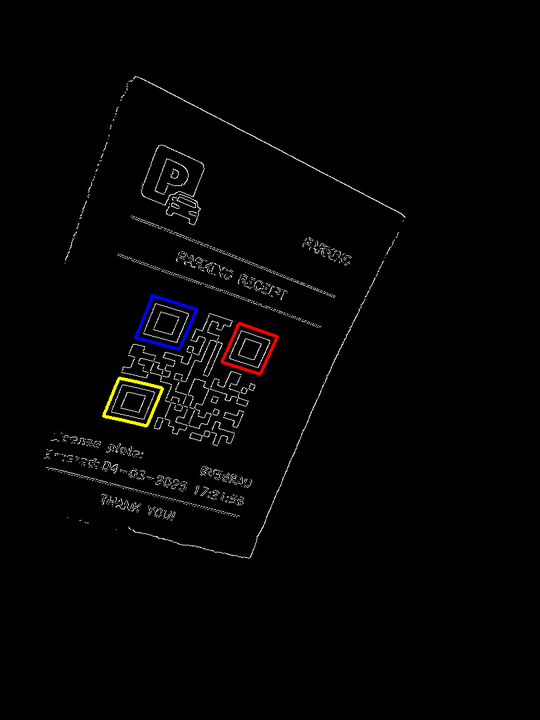
\includegraphics[width=0.25\textwidth]{images/anchors.png}
    \caption{Cele trei ancore QR detectate pe harta de margini obținută}
\end{figure}
\FloatBarrier

După calcularea scorurilor, candidații sunt sortați crescător după valoarea medie a similarității. Dacă există cel puțin trei candidați validați, sunt selectați primii trei, aceștia fiind considerați cele trei ancore ale codului QR.

\[
    anchors = \{C_1, C_2, C_3\}, \quad
    score(C_1) \leq score(C_2) \leq score(C_3)
\]

În cazul în care cele trei ancore sunt detectate cu succes, acestea trebuie ordonate în funcție de poziția lor în imagine. Pentru fiecare contur se calculează centrul de masă folosind momentele geometrice:

\[
    centroid =
    \left(
        \frac{m_{10}}{m_{00}},
        \frac{m_{01}}{m_{00}}
    \right)
\]

Cele trei ancore sunt apoi sortate în ancoră stânga-sus, ancoră dreapta-sus și ancoră stânga-jos. Clasificarea se face pe baza sumei și diferenței coordonatelor centrului de masă:

\[
p_{TL} = \arg\min_{p_i \in \mathcal{A}} (x_i + y_i)
\]

\[
p_{TR} = \arg\max_{p_i \in \mathcal{A}} (x_i - y_i)
\]

\[
p_{BL} = \arg\min_{p_i \in \mathcal{A}} (x_i - y_i)
\]

Această ordonare este necesară deoarece punctele de rectificare ale codului QR sunt calculate diferit pentru fiecare ancoră. Ancora din stânga-sus contribuie la determinarea colțului stânga-sus al codului, ancora din dreapta-sus contribuie la determinarea colțului dreapta-sus, iar ancora din stânga-jos contribuie la determinarea colțului stânga-jos.

Pentru fiecare ancoră detectată se extrage un bounding box local. Conturul ancorei este translatat în coordonate locale, apoi este desenat într-o imagine binară separată. În jurul acestei imagini se adaugă padding, astfel încât liniile detectate ulterior să nu fie întrerupte la marginea regiunii analizate.

\[
    paddingX = 0.4 \cdot bbox.width
\]

\[
    paddingY = 0.4 \cdot bbox.height
\]

Pe conturul astfel obținut se aplică transformata Hough probabilistică, cu scopul de a detecta segmentele de dreaptă care formează laturile marcatorului. Lungimea minimă a liniilor este inițial calculată în funcție de înălțimea bounding box-ului, iar distanța maximă dintre segmente este stabilită procentual față de aceeași dimensiune.

\[
    minLineLength = 0.8 \cdot bbox.height
\]

\[
    maxLineGap = 0.05 \cdot bbox.height
\]

Dacă liniile detectate nu pot fi sortate în cele patru laturi ale ancorei, valoarea pentru $minLineLength$ este decrementată treptat, iar transformata Hough este reaplicată. Astfel, algoritmul poate funcționa și în situații în care conturul este afectat de perspectivă, zgomot, blur sau întreruperi locale.
Liniile detectate trebuie sortate pentru a se obține câte o linie reprezentativă pentru fiecare latură: stânga, sus, dreapta și jos. Pentru început, liniile sunt separate în verticale și orizontale. Dacă o linie are aceeași coordonată X pentru ambele capete, aceasta este considerată direct verticală. În celelalte cazuri, se calculează panta și unghiul de înclinare:

\[
    slope = \frac{y_2 - y_1}{x_2 - x_1}
\]

\[
    angle = \left| \arctan(slope) \times \frac{180}{\pi} \right|
\]

Dacă unghiul este mai apropiat de $90^\circ$, linia este considerată verticală, iar dacă este mai apropiat de $0^\circ$, linia este considerată orizontală. Pentru liniile orizontale se calculează și panta medie, deoarece aceasta este folosită la construirea unei linii de referință care ține cont de eventuala înclinare a codului QR.

Pentru clasificarea liniilor în partea de sus, jos, stânga și dreapta, se construiesc două linii de referință care trec prin centrul imaginii: una orizontală și una verticală. Linia orizontală folosește panta medie calculată anterior, iar linia verticală este trasată prin același punct central. Aceste linii de referință sunt generate pe baza ecuației dreptei:

\[
    y = slope \cdot x + b
\]

\[
    b = y_0 - slope \cdot x_0
\]

unde $(x_0, y_0)$ este centrul imaginii. În funcție de direcția dorită, dreapta este extinsă fie între marginile stânga-dreapta ale imaginii, fie între marginile sus-jos.

Fiecare linie detectată este comparată cu linia de referință corespunzătoare. Pentru aceasta, se calculează punctul de mijloc al liniei detectate și se determină pe ce parte a liniei de referință se află. Semnul expresiei următoare stabilește clasificarea:

\[
    distance = (x - x_1) \cdot (y_2 - y_1) - (y - y_1) \cdot (x_2 - x_1)
\]

Dacă valoarea este pozitivă, segmentul este introdus într-un prim grup, iar în caz contrar într-un al doilea grup. Astfel, liniile orizontale sunt împărțite în linii de sus și linii de jos, iar liniile verticale sunt împărțite în linii din stânga și linii din dreapta.

În practică, pentru aceeași latură pot fi detectate mai multe segmente. Din acest motiv, segmentele din fiecare grup sunt unite într-o singură linie reprezentativă. Pentru aceasta, se caută punctul inițial cel mai îndepărtat și punctul terminal cel mai îndepărtat pe direcția analizată. Rezultatul este o aproximare a celor patru laturi ale marcatorului QR.

După obținerea liniilor sortate, se calculează punctele de intersecție dintre acestea. Pentru fiecare dintre cele trei ancore analizate se extrage câte un colț al codului QR: colțul stânga-sus, colțul dreapta-sus și colțul stânga-jos. Al patrulea colț, cel din dreapta-jos, este obținut prin intersectarea liniei din dreapta, memorată din ancora dreapta-sus, cu linia de jos, memorată din ancora stânga-jos. Calculul intersecției se face folosind forma generală a dreptei:

\[
    A x + B y = C
\]

Pentru două drepte, se calculează determinantul:

\[
    determinant = A_1 B_2 - A_2 B_1
\]

Dacă determinantul este diferit de zero, punctul de intersecție este calculat astfel:

\[
    x = \frac{B_2 C_1 - B_1 C_2}{determinant}, \quad
    y = \frac{A_1 C_2 - A_2 C_1}{determinant}
\]

\begin{figure}[htbp]
    \centering
    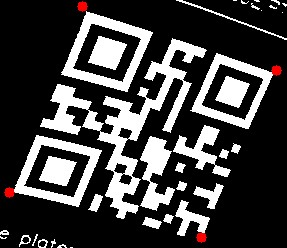
\includegraphics[width=0.3\textwidth]{images/qr12.jpg}
    \caption{Punctele de rectificare obținute din intersecția liniilor}
\end{figure}
\FloatBarrier

Înainte de rectificare, coordonatele sunt ușor extinse față de centrul regiunii. Se calculează centrul celor patru puncte, iar fiecare punct este deplasat spre exterior pe direcția vectorului dintre centru și punctul respectiv. Valoarea deplasării este un procent din dimensiunea minimă a imaginii. Această etapă ajută la includerea completă a codului QR în regiunea finală.

\[
    padding = percent \times \min(src.width, src.height)
\]

\[
    P_i = P_i + direction_i \times padding
\]

Există situații în care unele coordonate calculate pot ieși în afara imaginii. Pentru a evita pierderea acestor puncte, imaginea este extinsă prin adăugarea de padding în partea de sus, jos, stânga sau dreapta. După adăugarea padding-ului, coordonatele sunt actualizate astfel încât să corespundă noii imagini extinse. Implementarea verifică și faptul că imaginea extinsă nu depășește un procent maxim admis față de dimensiunea inițială

\[
    \begin{aligned}
        paddingRight  &= \max(0, maxX - (src.width - 1)), \\
        paddingBottom &= \max(0, maxY - (src.height - 1)), \\
        paddingLeft   &= \max(0, -minX), \\
        paddingTop    &= \max(0, -minY)
    \end{aligned}
\]

\[
    \begin{aligned}
        x &= x + paddingLeft, \quad
        y &= y + paddingTop
    \end{aligned}
\]

În final, se aplică transformarea geometrică propriu-zisă. Deoarece un cod QR are formă pătratică, imaginea destinație este construită cu lățimea egală cu înălțimea. Înălțimea este estimată pe baza diferenței dintre coordonata $y$ a punctului stânga-jos și coordonata $y$ a punctului stânga-sus:

\[
    height = DownLeft.y - UpLeft.y, \quad
    width = height
\]

Punctele sursă sunt asociate cu punctele corespondente din imaginea destinație:

\begin{itemize}
    \item $(0, 0)$ pentru colțul stânga-sus;
    \item $(width - 1, 0)$ pentru colțul dreapta-sus;
    \item $(0, height - 1)$ pentru colțul stânga-jos;
    \item $(width - 1, height - 1)$ pentru colțul dreapta-jos.
\end{itemize}

Pe baza acestor două seturi de puncte se calculează matricea de transformare perspectivă, iar regiunea candidată este transformată într-o imagine pătratică, aliniată frontal. Această imagine rectificată este folosită ulterior pentru extragerea matricei QR și pentru decodarea conținutului.

\begin{figure}[htbp]
    \centering
    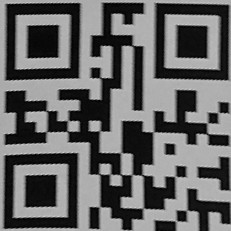
\includegraphics[width=0.3\textwidth]{images/qr13.jpg}
    \caption{Codul QR după transformarea geometrică}
\end{figure}
\FloatBarrier

După rectificarea geometrică a regiunii candidate, următorul pas constă în transformarea acesteia într-o reprezentare cât mai apropiată de matricea reală a codului QR. Imaginea rectificată este mai întâi redimensionată la dimensiunea $210 \times 210$ pixeli, folosind interpolare de tip \textit{nearest-neighbor}. Această metodă este potrivită în acest context deoarece păstrează muchiile clare dintre modulele albe și negre ale codului QR.

Imaginea redimensionată este apoi convertită într-un \textit{blob}, valorile pixelilor fiind normalizate prin împărțirea la $255$. Acest \textit{blob} este oferit ca input modelului neuronal, care are rolul de a reconstrui matricea binară a codului QR. Output-ul modelului este interpretat ca o matrice pătratică, dimensiunea acesteia fiind calculată pe baza numărului total de valori returnate.

\[
    n = \sqrt{output.total()}
\]

Dacă numărul total de valori nu poate forma o matrice pătratică, candidatul este respins. În caz contrar, output-ul este reorganizat într-o matrice de dimensiune $n \times n$ și este binarizat folosind pragul $0.5$.

\[
    pixel =
    \begin{cases}
        255, & \text{dacă } output > 0.5 \\
        0,   & \text{în caz contrar}
    \end{cases}
\]

\begin{figure}[htbp]
    \centering
    
\includegraphics[width=0.25\textwidth]{images/qr14.jpg}
    \caption{Matricea QR reconstruită de modelul neuronal}
\end{figure}
\FloatBarrier

După obținerea matricei binare, aceasta este transmisă bibliotecii \textit{ZXing}, care încearcă decodarea conținutului. Pentru a limita procesul strict la tipul de cod analizat, formatul de citire este setat explicit la \textit{QRCode}. Dacă decodarea nu produce un rezultat valid, regiunea candidată este eliminată.

În cazul în care decodarea reușește, textul extras este memorat ca identificator al tichetului sau al accesării.

\section{Modelul de rețea neuronală pentru decodarea codurilor QR}

Pentru decodarea codurilor QR, aplicația folosește un model de rețea neuronală care are rolul de a reconstrui matricea binară a codului QR dintr-o imagine afectată de perspectivă, scalare, rotație, blur, variații de contrast, zgomot, iluminare neuniformă sau alte defecte vizuale. Înainte de antrenarea modelului, a fost necesară generarea unui set de date sintetic, format din imagini QR și etichetele corespunzătoare fiecărei imagini.

Setul de date generat conține 40000 de imagini. Fiecare imagine reprezintă un cod QR de versiune 1, având dimensiunea logică de $21 \times 21$ module. Pentru a putea fi procesat mai ușor de model, fiecare cod QR este redimensionat la dimensiunea $210 \times 210$ pixeli, astfel încât fiecare modul al codului să fie reprezentat printr-un bloc de $10 \times 10$ pixeli.

Conținutul fiecărui cod QR este reprezentat de o dată și o oră generate aleatoriu, aflate în intervalul 1 ianuarie 2023 -- 31 decembrie 2026. Aceste valori sunt formatate sub forma:

\[
\text{zi-lună-an ora:minut:secundă}
\]

Pentru fiecare dată generată se obține și un nume unic de fișier, construit pe baza aceleiași valori temporale, dar fără separatori. Astfel, fiecare imagine din setul de date are asociat un fișier text cu aceeași denumire, care conține eticheta corespunzătoare.

\begin{figure}[htbp]
\centering
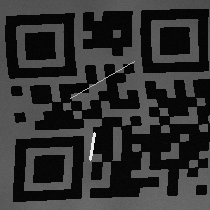
\includegraphics[width=0.25\textwidth]{images/data_exemple.png}
\caption{Exemplu de imagine generată pentru setul de date}
\end{figure}
\FloatBarrier

Pentru generarea codului QR se folosește o bibliotecă dedicată, configurată pentru coduri QR de versiune 1, cu nivel de corecție a erorilor de tip \textit{M}. Codul este generat fără margine suplimentară, astfel încât imaginea rezultată să conțină strict matricea QR propriu-zisă. Matricea logică a codului este salvată separat și reprezintă eticheta folosită la antrenare.

Eticheta fiecărei imagini este un fișier text ce conține matricea codului QR, unde fiecare valoare indică starea unui modul:

\[
    label_{i,j} =
    \begin{cases}
        1, & \text{dacă modulul este negru} \\
        0, & \text{dacă modulul este alb}
    \end{cases}
\]

În acest fel, modelul nu este antrenat să recunoască direct textul din codul QR, ci să reconstruiască structura binară a codului. Decodarea textului este realizată ulterior, folosind matricea prezisă de model.

Pentru ca modelul să fie robust la situații întâlnite în imagini reale, fiecare cod QR generat este augmentat printr-o succesiune de transformări geometrice și fotometrice. Înainte de aplicarea acestor transformări, imaginea este redimensionată la dimensiunea standard de $210 \times 210$ pixeli.

Prima etapă de augmentare modifică marginea imaginii prin aplicarea unei operații de padding sau crop. Valorile sunt alese aleatoriu pentru fiecare latură, într-un interval proporțional cu dimensiunea imaginii. Astfel, codul QR poate fi ușor deplasat, încadrat imperfect sau tăiat marginal, simulând situații în care regiunea detectată nu corespunde exact codului QR.

Următoarea transformare este rotația aleatorie. Cu o anumită probabilitate, imaginea este rotită cu un unghi ales în intervalul $[-8^\circ, 8^\circ]$, iar în același timp poate fi scalată ușor, cu un factor apropiat de valoarea $1$. Zonele apărute în afara imaginii sunt completate cu valori luminoase, apropiate de fundalul unei foi sau al unei suprafețe deschise la culoare.

Se aplică apoi o transformare de perspectivă, prin care colțurile imaginii sunt deplasate ușor în interiorul acesteia. Această etapă simulează cazul în care codul QR este fotografiat dintr-un unghi diferit de cel frontal. Deformarea este controlată printr-o margine aleatorie raportată la dimensiunea imaginii, astfel încât structura codului să rămână recognoscibilă.

Pentru a simula curbarea sau deformarea ușoară a suprafeței pe care se află codul QR, se aplică o transformare sinusoidală asupra coordonatelor pixelilor. Această augmentare deplasează pixelii pe axele Ox și Oy folosind funcții sinusoidale cu amplitudine, frecvență și fază alese aleatoriu. În acest mod, imaginea poate semăna cu un cod QR imprimat pe o suprafață ușor curbată sau fotografiat în condiții imperfecte.

Următoarea augmentare este scalarea anizotropică. Imaginea este scalată diferit pe axele Ox și Oy, folosind factori aleatori apropiați de valoarea $1$. Astfel, codul QR poate deveni ușor întins sau comprimat pe una dintre direcții, simulând erori de rectificare sau deformări apărute în procesul de captare. După această etapă, imaginea este din nou redimensionată la dimensiunea standard de $210 \times 210$ pixeli.

După transformările geometrice se aplică operații morfologice. Aleatoriu, imaginea poate fi procesată prin eroziune, dilatare, deschidere sau închidere morfologică, folosind un kernel de dimensiune mică. Aceste operații modifică grosimea modulelor negre sau reduc/închid goluri locale, simulând efecte produse de imprimare, compresie, focalizare imperfectă sau praguri de binarizare diferite.

Pentru simularea fundalului real al unei imagini, zonele albe ale codului QR sunt înlocuite cu un fundal gri, peste care se adaugă zgomot fin și textură de frecvență joasă. Nivelul de gri este ales aleatoriu, iar textura este generată prin zgomot gaussian și printr-o hartă de intensitate interpolată la dimensiunea imaginii. Astfel, fundalul nu rămâne perfect alb, ci capătă variații asemănătoare unei suprafețe reale.

În mod similar, modulele negre sunt modificate printr-o operație de ridicare a nivelului de negru. În loc să fie reprezentate mereu prin valoarea $0$, zonele întunecate pot primi valori mai mari, peste care se adaugă zgomot. Această etapă simulează situațiile în care codul QR este slab imprimat, supraexpus sau afectat de reflexii.

Pentru a simula condițiile diferite de iluminare, se aplică o mască de lumină neuniformă. Aceasta este construită în funcție de distanța față de un centru ales aleatoriu și poate produce zone mai luminoase sau mai întunecate în imagine. În unele cazuri, se adaugă și o bandă luminoasă verticală, care poate simula reflexii sau iluminare direcțională. La final, întreaga imagine este modificată printr-un factor global de intensitate și printr-o deplasare aleatorie a luminozității.

Pentru a simula neclaritatea produsă de mișcare, focalizare imperfectă sau calitatea camerei, se aplică aleatoriu și blur. Acesta poate fi de tip Gaussian, cu mască și deviație standard alese aleatoriu, sau ca tip de neclaritate de mișcare, folosind o mască orientat orizontal sau vertical. Această etapă obligă modelul să învețe structura generală a codului QR, nu doar tranzițiile perfect clare dintre pixeli.

O altă augmentare modifică nivelul de contrast și luminozitate al imaginii. Factorul de contrast este ales aleatoriu, iar peste imagine se adaugă o variație de luminozitate. Această etapă simulează condiții diferite de expunere, precum umbre, reflexii sau iluminare neuniformă.

Peste imagine se poate adăuga și zgomot. În unele cazuri se folosește zgomot gaussian, iar în altele se adaugă zgomot de tip sare și piper, prin care anumiți pixeli sunt transformați în valori foarte întunecate sau foarte luminoase. Această etapă simulează artefacte produse de senzorul camerei, compresie sau zgomot digital.

Pentru a simula defecte ale hârtiei sau ale suprafeței pe care se află codul QR, se pot desena aleatoriu linii subțiri peste imagine. Acestea au poziții, lungimi, intensități și grosimi diferite, reprezentând zgârieturi, urme, cute sau alte imperfecțiuni locale.

Ultima etapă de augmentare poate aplica o compresie JPEG cu o calitate aleatorie. Imaginea este codificată temporar în format JPEG și apoi decodificată înapoi în nuanțe de gri. Această transformare introduce artefacte specifice compresiei, întâlnite frecvent în imagini salvate sau transmise prin aplicații externe.

În urma acestor pași, fiecare imagine din setul de date conține un cod QR distorsionat controlat, iar fiecare etichetă conține matricea QR ideală, fără distorsiuni. Această abordare permite modelului să învețe să transforme o imagine imperfectă într-o reprezentare binară corectă, care poate fi apoi transmisă mai departe către etapa de decodare.

În continuare, este definită arhitectura modelului utilizat pentru reconstrucția matricei binare a codului QR. Modelul este construit ca o rețea convoluțională compactă, adaptată special pentru problema identificării celor $21 \times 21$ module ale unui cod QR de versiune 1.

Scopul modelului nu este de a recunoaște direct textul codificat în QR, ci de a prezice valoarea fiecărui modul din matricea QR. Astfel, pentru o imagine de intrare de dimensiune $210 \times 210$, modelul produce o matrice de ieșire de dimensiune $21 \times 21$.

\begin{figure}[htbp]
\centering
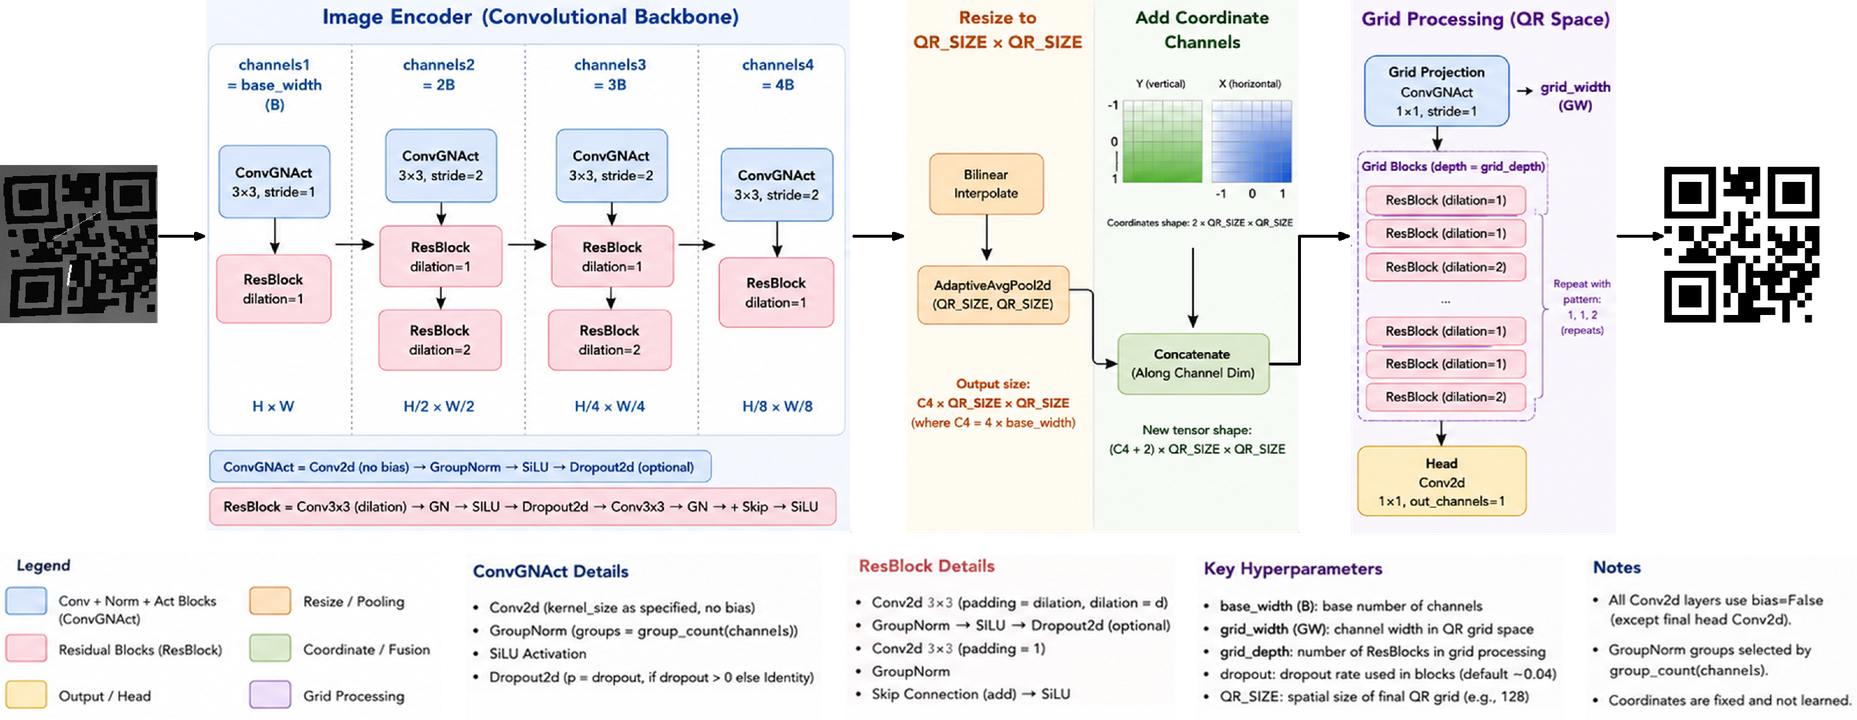
\includegraphics[width=0.85\textwidth]{images/arhitecture.png}
\caption{Arhitectura modelului}
\end{figure}
\FloatBarrier

Imaginea de intrare este încărcată în nuanțe de gri și normalizată prin împărțirea valorilor pixelilor la $255$. Astfel, fiecare pixel ajunge să aibă o valoare în intervalul $[0, 1]$. Deoarece imaginea are un singur canal, tensorul de intrare are forma:

\[
x \in \mathbb{R}^{1 \times 210 \times 210}
\]

Pentru antrenare, fiecare imagine are asociată o etichetă de dimensiune $21 \times 21$, care reprezintă matricea logică reală a codului QR. Fiecare element al acestei matrice indică dacă modulul corespunzător este alb sau negru.

Arhitectura modelului este formată din două părți principale: un encoder convoluțional pentru extragerea caracteristicilor din imagine și o secțiune de procesare la nivel de grilă, care produce predicția finală pentru fiecare modul QR.

Primul bloc folosit în model conține un strat convoluțional, urmat de o normalizare pe grupuri, funcția de activare \textit{SiLU} și, opțional, o etapă de anulare aleatorie a unor canale prin \textit{Dropout2d}. Convoluția este aplicată fără termen liber, deoarece normalizarea ulterioară compensează deplasarea valorilor intermediare.

\[
    h = SiLU(GN(Conv(x)))
\]

Funcția de activare folosită este \textit{SiLU}, definită astfel:

\[
    SiLU(x) = x \cdot \sigma(x)
\]

unde $\sigma(x)$ este funcția sigmoidă.

Pentru normalizare se folosește normalizarea pe grupuri. Aceasta împarte canalele tensorului în mai multe grupuri și normalizează valorile în interiorul fiecărui grup. Numărul de grupuri este ales automat, în funcție de numărul de canale, preferându-se valoarea $8$ atunci când aceasta divide numărul de canale. Această alegere face ca modelul să fie mai stabil la antrenare, inclusiv pentru loturi de dimensiune mai mică, deoarece normalizarea nu depinde direct de statisticile întregului lot.

Encoderul imaginii pornește de la un canal de intrare și crește treptat numărul de canale. În implementarea curentă, lățimea de bază este $32$, iar canalele intermediare sunt:

\[
32,\ 64,\ 96,\ 128
\]

Prima etapă păstrează rezoluția imaginii și extrage caracteristici de nivel jos, precum muchii, zone întunecate, tranziții între module și variații locale de intensitate. Următoarele etape folosesc convoluții cu pas $2$, reducând treptat rezoluția spațială și crescând numărul de canale. Astfel, modelul obține o reprezentare mai compactă și mai bogată semantic a imaginii.

Encoderul conține și blocuri reziduale. Un bloc rezidual primește un tensor cu un anumit număr de canale și returnează un tensor cu aceeași dimensiune. Fiecare bloc este alcătuit din două straturi convoluționale cu kernel $3 \times 3$, normalizare pe grupuri, activare \textit{SiLU} și o conexiune reziduală între intrare și ieșire.

\[
y = SiLU(x + F(x))
\]

unde $F(x)$ reprezintă transformarea învățată de cele două straturi convoluționale din bloc.

În unele blocuri reziduale se folosesc convoluții dilatate. Acestea măresc câmpul receptiv al modelului fără a reduce rezoluția spațială a reprezentării. În contextul codurilor QR, acest lucru este util deoarece decizia pentru un modul poate depinde de vecinătatea sa și de structurile regulate ale codului, precum marcatorii de poziționare sau modelele de sincronizare.

\[
\begin{aligned}
h &= SiLU(GN(Conv_{3 \times 3}^{d}(x))) \
h &= GN(Conv_{3 \times 3}(h)) \
y &= SiLU(x + h)
\end{aligned}
\]

unde $d$ reprezintă factorul de dilatare al primei convoluții din bloc.

După encoderul convoluțional, reprezentarea este adusă la dimensiunea logică a codului QR. Pentru aceasta, se folosește interpolare biliniară până la rezoluția $21 \times 21$:

\[
H \times W \rightarrow 21 \times 21
\]

Această etapă transformă caracteristicile extrase din imagine într-o reprezentare aliniată cu grila QR. Fiecare poziție din această grilă corespunde unui modul al codului QR.

Pentru a oferi modelului informație explicită despre poziția fiecărui modul în matrice, se construiesc două hărți de coordonate, corespunzătoare axelor verticală și orizontală. Valorile acestora sunt distribuite în intervalul $[-1, 1]$ și au dimensiunea $21 \times 21$. Cele două hărți sunt concatenate cu tensorul de caracteristici înainte de procesarea la nivel de grilă.

\[
x_{grid} = [x,\ coord_y,\ coord_x]
\]

Această informație pozițională este importantă deoarece un cod QR nu are aceeași semnificație în toate zonele sale. De exemplu, colțurile conțin marcatori de poziționare, iar anumite linii conțin modele de sincronizare. Prin includerea coordonatelor, modelul poate învăța mai ușor comportamente diferite pentru regiuni diferite ale matricei QR.

După concatenarea coordonatelor, tensorul este trecut printr-o proiecție convoluțională de tip $1 \times 1$, care transformă numărul de canale în $128$. Această etapă produce reprezentarea principală folosită de secțiunea de procesare la nivel de grilă.

\[
\mathbb{R}^{130 \times 21 \times 21}
\rightarrow
\mathbb{R}^{128 \times 21 \times 21}
\]

Partea principală a procesării pe grilă este formată din $6$ blocuri reziduale. Acestea păstrează rezoluția spațială de $21 \times 21$ și lucrează cu $128$ de canale. Unele dintre aceste blocuri folosesc dilatare, ceea ce permite modelului să combine informații dintr-o vecinătate mai largă fără a pierde corespondența cu modulele QR.

Această succesiune de blocuri reziduale rafinează reprezentarea fiecărui modul, ținând cont atât de conținutul local al imaginii, cât și de relațiile spațiale dintre module. În contextul codurilor QR, acest lucru este relevant deoarece matricea nu este o colecție de biți complet independenți. Există structuri locale clare, cum ar fi marcatorii de poziționare, marginile și modelele de sincronizare, iar modelul poate exploata aceste relații spațiale pentru a reconstrui mai corect matricea finală.

La finalul blocurilor reziduale se aplică un strat convoluțional de tip $1 \times 1$, care reduce numărul de canale de la $128$ la $1$. Acest strat funcționează ca un cap de clasificare aplicat fiecărei poziții din matricea $21 \times 21$. Pentru fiecare modul QR, modelul produce o valoare reală, numită valoare logit.

\[
\mathbb{R}^{128 \times 21 \times 21}
\rightarrow
\mathbb{R}^{1 \times 21 \times 21}
\]

După eliminarea dimensiunii canalului, ieșirea finală a modelului are forma:

\[
output \in \mathbb{R}^{21 \times 21}
\]

În timpul antrenării, aceste scoruri brute, numite și valori logit, sunt comparate cu matricea reală a codului QR folosind funcția de cost \textit{entropie încrucișată binară cu logiți}. Această funcție este potrivită deoarece fiecare poziție din matrice reprezintă o decizie binară: modul alb sau modul negru.

\[
\mathcal{L} =
- \left[
y \cdot \log(\sigma(z)) +
(1-y) \cdot \log(1-\sigma(z))
\right]
\]

unde $z$ este logitul produs de model, $y$ este valoarea reală a modulului, iar $\sigma(z)$ este probabilitatea obținută prin aplicarea funcției sigmoid.

Setul de date este împărțit în două subseturi: $80\%$ pentru antrenare și $20\%$ pentru validare. Împărțirea este realizată aleatoriu, dar reproductibil, folosind o sămânță fixă. Imaginile sunt procesate în batch-uri de câte $32$, ceea ce permite antrenarea eficientă a modelului și o estimare stabilă a gradientului la fiecare pas.

Optimizarea se realizează folosind algoritmul \textit{AdamW}, cu o rată de învățare de $10^{-4}$ și regularizare prin penalizarea greutăților cu valoarea $10^{-4}$. Pentru stabilitate numerică, optimizatorul folosește valoarea $\varepsilon = 10^{-7}$. Alegerea algoritmului \textit{AdamW} este potrivită pentru acest tip de model deoarece combină adaptarea automată a ratei de învățare pentru fiecare parametru cu o regularizare mai stabilă a greutăților.

Antrenarea se realizează pentru maximum $50$ de epoci. După fiecare epocă, modelul este evaluat pe setul de validare, iar rata de învățare este ajustată printr-un planificator de tip \textit{ReduceLROnPlateau}. Acesta urmărește acuratețea exactă pe validare și reduce rata de învățare cu un factor de $0.5$ dacă performanța nu se îmbunătățește timp de mai multe epoci. Rata minimă de învățare este limitată la $2 \cdot 10^{-6}$.

Pentru a evita instabilitățile apărute în urma unor gradienți prea mari, se folosește limitarea normei gradientului. Norma gradientului este limitată la valoarea $0.5$, iar pașii de optimizare sunt evitați dacă apar valori numerice nefinite. În timpul antrenării sunt verificate atât imaginile și etichetele, cât și valoarea funcției de cost și norma gradientului, pentru a preveni propagarea unor valori invalide prin rețea.
Modelul poate relua antrenarea dintr-un checkpoint existent. Dacă fișierul cu greutățile modelului este găsit, se încarcă starea rețelei, cea mai bună acuratețe pe biți, cea mai bună acuratețe exactă și epoca de la care trebuie continuată antrenarea. Astfel, procesul poate fi întrerupt și reluat fără pierderea progresului anterior.

Performanța modelului este măsurată prin două metrici. Prima este acuratețea la nivel de bit, care indică procentul de module QR prezise corect:

\[
Acc_{bit} =
\frac{\text{numărul de module prezise corect}}
{\text{numărul total de module}}
\]

A doua este acuratețea exactă la nivel de imagine, care verifică dacă întreaga matrice $21 \times 21$ a fost prezisă corect. O imagine este considerată corectă doar dacă toate cele $441$ de module au valoarea corectă:

\[
Acc_{exact} =
\frac{\text{numărul de imagini reconstruite complet corect}}
{\text{numărul total de imagini}}
\]

Checkpoint-ul final este salvat atunci când modelul obține o acuratețe exactă mai bună pe setul de validare. În cazul unei egalități la acuratețea exactă, este preferat modelul cu acuratețe mai bună la nivel de bit. În fișierul salvat se păstrează starea modelului, epoca, cele mai bune valori ale metricilor și configurația principală folosită pentru antrenare.

După antrenare, modelul este împachetat într-o clasă auxiliară care aplică funcția sigmoid peste logiți și transformă probabilitățile în biți. În această etapă, fiecare valoare este comparată cu pragul $0.5$, iar rezultatul final este o matrice binară.

\[
p = \sigma(z)
\]

\[
    bit =
    \begin{cases}
        1, & \text{dacă } p > 0.5 \\
        0, & \text{în caz contrar}
    \end{cases}
\]

Rezultatul final este exportat în format ONNX, pentru a putea fi încărcat ulterior în aplicația C++ prin modulul \textit{OpenCV DNN}. Exportul folosește un input de forma:

\[
image \in \mathbb{R}^{1 \times 1 \times 210 \times 210}
\]

iar ieșirea modelului este o matrice de biți. Pentru export se folosește opset-ul $17$, iar axa batch-ului este definită dinamic, astfel încât modelul exportat să poată procesa atât o singură imagine, cât și mai multe imagini simultan.

Prin această arhitectură, modelul funcționează ca un reconstructor de matrice QR: primește o imagine distorsionată sau imperfectă a codului și produce o matrice binară curată, care poate fi transmisă mai departe către biblioteca de decodare.

\section{Serverul HTTP și gestionarea cererilor}

Serverul HTTP reprezintă componenta centrală responsabilă pentru comunicarea dintre aplicația web și logica internă a sistemului. Acesta expune funcționalitățile aplicației printr-o serie de endpoint-uri REST, permițând clienților să efectueze operații precum autentificarea, crearea conturilor, administrarea abonamentelor, gestionarea vehiculelor, validarea plăților și transmiterea mesajelor.

Serverul este implementat utilizând biblioteca \textit{cpp-httplib}, care permite definirea rapidă a endpoint-urilor și gestionarea eficientă a cererilor HTTP. Acesta rulează pe portul 8080 și acceptă conexiuni pe toate interfețele de rețea, oferind acces atât local, cât și din exterior.

\begin{figure}[htbp]
    \centering
    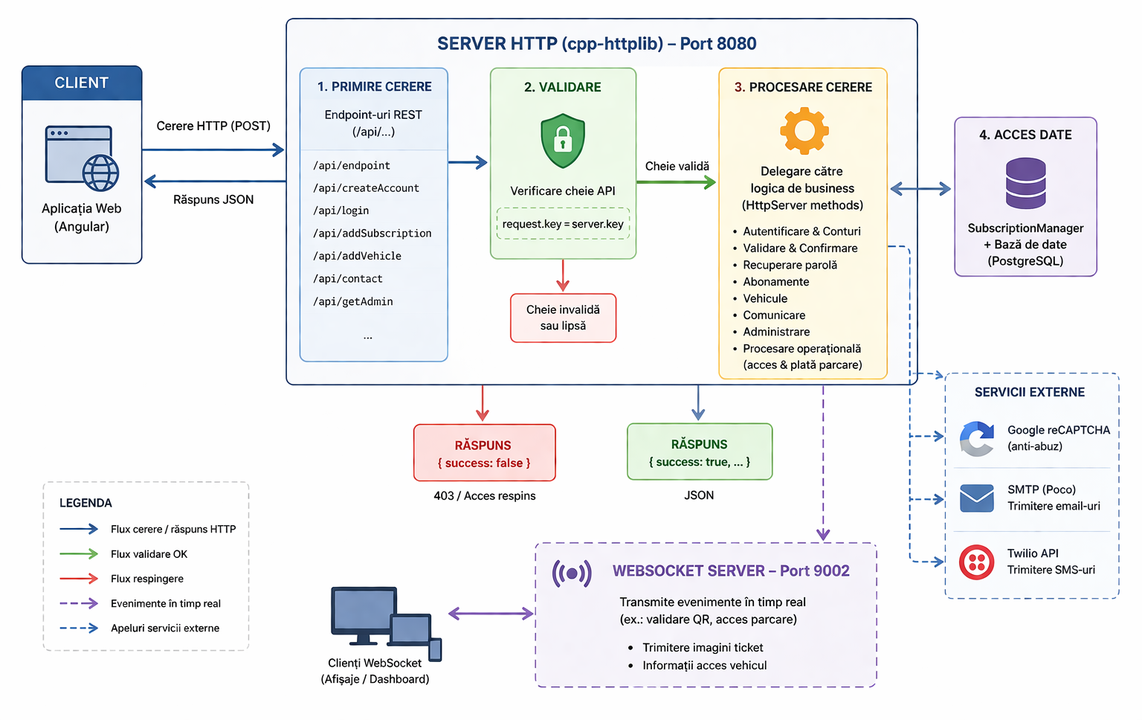
\includegraphics[width=0.85\textwidth]{images/http.png}
    \caption{Fluxul general de comunicare prin serverul HTTP}
\end{figure}
\FloatBarrier

La inițializare, serverul configurează cheia de acces utilizată pentru validarea cererilor și adresa aplicației web. În modul de dezvoltare, aceste valori sunt definite local, iar în producție sunt preluate din variabile de mediu, evitând expunerea datelor sensibile în cod.

Fiecare cerere trebuie să conțină parametrul \textit{key}, iar validarea se face astfel:

\[
    request.key = server.key
\]

Dacă cheia este invalidă sau lipsește, cererea este respinsă imediat:

\[
    response = \{success: false\}
\]

Acest mecanism oferă un nivel de protecție împotriva accesului neautorizat.

Toate endpoint-urile sunt definite ca cereri și sunt organizate pe categorii funcționale, în funcție de rolul pe care îl au în cadrul aplicației:

\begin{itemize}
    \item \textbf{Autentificare și administrarea conturilor:} această categorie gestionează crearea conturilor, autentificarea utilizatorilor, validarea conturilor temporare și actualizarea informațiilor personale, precum numele, prenumele, telefonul, e-mailul sau parola.

    \item \textbf{Validare și confirmare identitate:} aceste cereri sunt utilizate pentru confirmarea acțiunilor importante prin e-mail sau SMS. Serverul generează token-uri numerice, le asociază conturilor temporare sau modificărilor cerute și le transmite utilizatorului prin serviciile externe configurate.

    \item \textbf{Recuperarea parolei:} această categorie permite inițierea procesului de resetare a parolei, trimiterea unui cod sau a unui link de resetare, verificarea token-ului primit și actualizarea parolei contului.

    \item \textbf{Gestionarea abonamentelor:} endpoint-urile din această zonă permit adăugarea, ștergerea și consultarea abonamentelor asociate unui cont. De asemenea, serverul poate returna vehiculele legate de un anumit abonament.

    \item \textbf{Gestionarea vehiculelor:} această categorie se ocupă cu adăugarea și eliminarea vehiculelor din abonamente, normalizarea numerelor de înmatriculare și afișarea istoricului unui vehicul, incluzând timpul petrecut în parcare și suma de plată.

    \item \textbf{Comunicare cu utilizatorii:} aceste cereri acoperă trimiterea mesajelor de contact, răspunsurile automate și gestionarea abonării sau dezabonării de la newsletter.

    \item \textbf{Administrare:} această categorie oferă funcționalități specifice administratorului, precum obținerea listei de utilizatori existenți în sistem și verificarea separată a credențialelor de administrator.

    \item \textbf{Procesare operațională a parcării:} această parte gestionează fluxul principal al sistemului, adică validarea accesului și plata parcării pe baza numărului de înmatriculare sau a unui cod QR, cu transmiterea evenimentelor relevante prin WebSocket.
\end{itemize}

Fiecare endpoint delegă logica către metode din clasa \textit{HttpServer}, asigurând separarea între rutare și logica de business.

Toate răspunsurile sunt returnate în format JSON, utilizând biblioteca \textit{nlohmann::json}. Structura generală este:

\[
    response =
    \begin{cases}
        \{success: true, \ldots\}, & \text{dacă operația reușește} \\
        \{success: false, \ldots\}, & \text{dacă operația eșuează}
    \end{cases}
\]

Răspunsurile pot conține date suplimentare: informații despre cont, abonamente, vehicule sau rezultate ale procesării.

Endpoint-ul \texttt{/api/endpoint} gestionează accesul vehiculelor în parcare și suportă două tipuri de input:

\begin{itemize}
    \item număr de înmatriculare;
    \item imagine cu cod QR.
\end{itemize}

Numărul de înmatriculare este normalizat (majuscule) și verificat în baza de date. În cazul unui cod QR, acesta este decodificat și transformat într-un timestamp utilizat pentru validarea plății.

Dacă plata este validă, serverul returnează informații despre vehicul și momentul intrării. În cazul codurilor QR, datele sunt transmise și prin WebSocket către clienți.

Crearea unui cont implică validarea reCAPTCHA și verificarea unicității emailului și telefonului. Contul este inițial temporar și necesită validare printr-un cod:

\[
    token \in [100000, 999999]
\]

Validarea se face prin email (SMTP - Poco) sau SMS (Twilio API). După confirmare, contul devine permanent. Autentificarea verifică credențialele și returnează datele contului și abonamentele asociate. Serverul suportă resetarea parolei prin email sau SMS, utilizând token-uri temporare. După validarea token-ului, parola poate fi actualizată în siguranță.

Utilizatorii pot administra abonamentele și vehiculele prin endpoint-uri dedicate. Numerele de înmatriculare sunt normalizate pentru consistență, iar rezultatele sunt returnate sub formă de tabele JSON. Există și endpoint-uri care oferă istoricul complet al unui vehicul, inclusiv timpul petrecut în parcare și costurile asociate.

Serverul utilizează servicii externe pentru funcționalități extinse:
\begin{itemize}
    \item \textbf{Google reCAPTCHA} – prevenirea abuzurilor;
    \item \textbf{SMTP (Poco)} – trimitere email-uri;
    \item \textbf{Twilio API} – trimitere SMS-uri.
\end{itemize}

Toate credențialele sunt gestionate prin variabile de mediu și pentru fiecare endpoint sunt implementate verificări riguroase:
\begin{itemize}
    \item validarea parametrilor;
    \item verificarea consistenței datelor;
    \item tratarea excepțiilor.
\end{itemize}

În caz de eroare, serverul loghează evenimentul și returnează un răspuns controlat.

În concluzie, serverul HTTP reprezintă nucleul sistemului, asigurând comunicarea între componente, validarea cererilor, integrarea cu servicii externe și transmiterea datelor în timp real.

\section{Serverul WebSocket pentru comunicații în timp real}

Serverul WebSocket reprezintă componenta responsabilă pentru schimbul rapid de informații între server și aplicația desktop. Spre deosebire de comunicarea HTTP, unde fiecare operație presupune o cerere separată inițiată de client, WebSocket-ul menține o conexiune deschisă între cele două componente. Astfel, serverul poate transmite imediat evenimente către client, fără a fi necesare interogări repetate.

În cadrul aplicației, serverul WebSocket este implementat folosind bibliotecile \textit{Boost.Asio} și \textit{Boost.Beast}. \textit{Boost.Asio} gestionează operațiile asincrone de rețea, iar \textit{Boost.Beast} oferă suport pentru protocolul WebSocket. Serverul acceptă conexiuni TCP, citește cererea inițială HTTP de upgrade și, dacă aceasta este validă, transformă conexiunea într-o sesiune WebSocket activă.

La conectare, clientul transmite un token in URL. Serverul extrage acest token din adresa cererii și îl compară cu valoarea configurată în variabilele de mediu. Dacă token-ul nu este valid, conexiunea este închisă imediat, fără acceptarea sesiunii WebSocket.

Serverul permite existența unei singure sesiuni active la un moment dat. Dacă există deja un client conectat, orice nouă conexiune este respinsă. Această decizie este potrivită pentru scenariul aplicației, unde componenta desktop reprezintă punctul principal de control al parcării, iar comunicarea în timp real trebuie realizată cu o singură instanță activă.

După acceptarea conexiunii se gestionează citirea, scrierea și închiderea sesiunii. Comunicarea este realizată asincron: serverul apelează permanent funcția de citire, iar după fiecare mesaj primit construiește un răspuns și reia ascultarea pentru următorul mesaj.

Mesajele transmise prin WebSocket sunt reprezentate în format JSON. Fiecare cerere conține un câmp care indică operația dorită, și un câmp folosit pentru asocierea răspunsului cu cererea inițială. Structura generală a unei cereri este:

\[
    request = \{command, requestId, \ldots\}
\]

Serverul construiește pentru fiecare cerere un răspuns de tip:

\[
    response = \{type, command, requestId, status, \ldots\}
\]

Comenzile tratate de server sunt următoarele:

\begin{itemize}
    \item funcționalitate care permite obținerea listei vehiculelor existente în baza de date;
    \item funcționalitate care permite adăugarea unui vehicul nou, împreună cu data, tichetul asociat și suma totală;
    \item funcționalitate care verifică dacă pentru un anumit vehicul a fost efectuată plata;
    \item funcționalitate care permite obținerea listei tichetelor existente în sistem.
\end{itemize}

Pentru fiecare dintre aceste comenzi, serverul apelează metodele corespunzătoare, astfel, WebSocket-ul nu implementează direct logica de persistență, ci funcționează ca un canal de comunicare între client și componenta responsabilă cu baza de date.

Un rol important al serverului WebSocket este transmiterea tichetelor generate în urma procesării imaginilor sau a codurilor QR. Serverul salvează tichetul în baza de date, generează un identificator intern pentru acesta și transmite către client un mesaj. Imaginea asociată tichetului este convertită în Base64 pentru a putea fi inclusă în mesajul JSON.

Structura unui astfel de mesaj este:

\[
    ticket = \{type, ticketId, image, id, licensePlate, dateTime\}
\]

Pentru trimiterea mesajelor, sesiunea folosește o coadă internă de scriere. Atunci când un mesaj trebuie transmis, acesta este introdus în coadă, iar dacă nu există deja o operație de scriere în desfășurare, se pornește trimiterea asincronă. După finalizarea unei scrieri, mesajul este eliminat din coadă, iar dacă mai există mesaje, este pornită următoarea trimitere. Această abordare previne suprapunerea operațiilor de scriere pe aceeași conexiune WebSocket.

\[
    writeQueue = [message_1, message_2, \ldots, message_n]
\]

În cazul apariției unei erori la citire sau scriere, sesiunea este închisă controlat. Conexiunea TCP este oprită, coada de mesaje este golită, iar callback-ul de închidere resetează sesiunea activă din server. Astfel, serverul poate accepta ulterior o nouă conexiune validă.

Prin utilizarea WebSocket-ului, aplicația poate transmite rapid informații operaționale între server și componenta desktop. Acest mecanism este esențial pentru scenariile în care evenimentele trebuie propagate imediat, cum ar fi generarea unui tichet, verificarea stării de plată sau actualizarea listei de vehicule. În acest fel, sistemul evită interogările periodice inutile și oferă o comunicare eficientă, bidirecțională și adaptată cerințelor unei aplicații de monitorizare în timp real.

\section{Securizarea și criptarea datelor}

Pentru protejarea comunicației dintre server și aplicația desktop, mesajele transmise prin WebSocket nu sunt trimise direct în format JSON lizibil, ci sunt serializate, criptate și apoi codificate într-o formă sigură pentru transmitere ca text. Această etapă este importantă deoarece prin WebSocket sunt schimbate informații operaționale ale sistemului, precum lista vehiculelor, starea plății, datele tichetelor sau imaginile asociate acestora.

Mecanismul de criptare este implementat atât în server, cât și în clientul WebSocket, folosind aceeași logică de codificare și decodificare. Mesajul JSON este mai întâi transformat într-un șir de caractere, după care este transmis funcției de criptare. La recepție, mesajul este decriptat și reconstruit.

Criptarea se bazează pe algoritmul AES cu o cheie de 256 de biți. Implementarea verifică faptul că aceasta are exact 32 de caractere, adică 32 de octeți, dimensiunea necesară pentru AES-256. Dacă această condiție nu este îndeplinită, mesajul nu este criptat sau decriptarea returnează un obiect JSON gol.

\[
    key.length = 32 \ bytes = 256 \ bits
\]

Înainte de criptare, textul este completat astfel încât dimensiunea sa să fie multiplu de 16 octeți, deoarece AES procesează datele în blocuri fixe de 128 de biți. Padding-ul folosit adaugă la final un număr de caractere egal cu numărul de octeți necesari pentru completarea ultimului bloc.

\[
    padding = 16 - (text.length \bmod 16)
\]

\[
    paddedText = text + padding \times char(padding)
\]

După adăugarea padding-ului, mesajul este parcurs în blocuri de câte 16 octeți. Fiecare bloc este criptat folosind cheia AES, iar rezultatele sunt concatenate într-un singur șir binar. Deoarece rezultatul criptării poate conține caractere care nu pot fi transmise în siguranță ca text prin WebSocket sau incluse direct în JSON, acesta este codificat ulterior în format Base64.

\[
    cipherText = AES(block_1) \Vert AES(block_2) \Vert \ldots \Vert AES(block_n)
\]

\[
    message = Base64(cipherText)
\]

Procesul invers are loc la recepția mesajului. Mai întâi, textul primit este decodificat din Base64, obținându-se din nou șirul binar criptat. Apoi se verifică dacă dimensiunea acestuia este validă, adică nenulă și multiplu de 16 octeți. Dacă această condiție nu este respectată, mesajul este considerat invalid.

\[
    cipherText.length \bmod 16 = 0
\]

Fiecare bloc criptat este decriptat folosind aceeași cheie AES, iar blocurile rezultate sunt concatenate pentru a obține textul inițial cu padding. Ultimul octet indică dimensiunea padding-ului, iar implementarea verifică dacă această valoare se află în intervalul valid, între 1 și 16. Dacă padding-ul este valid, acesta este eliminat, iar textul rămas este interpretat ca JSON.

\[
    padding \in [1, 16]
\]

\[
    text = decryptedText[0, decryptedText.length - padding]
\]

Acest mecanism este folosit pentru toate mesajele principale schimbate prin WebSocket. De exemplu, atunci când clientul trimite o cerere către server, obiectul JSON primește câmpurile, apoi este criptat înainte de transmitere. Serverul decriptează mesajul, extrage comanda cerută, execută operația corespunzătoare și trimite înapoi un răspuns criptat.

Pe partea serverului, același principiu este folosit și pentru trimiterea tichetelor. Imaginea asociată tichetului este convertită în Base64, deoarece reprezintă date binare, apoi este inclusă într-un obiect JSON alături de identificatorul tichetului, numărul de înmatriculare și data generării. Întregul obiect este serializat și criptat înainte de a fi introdus în coada de trimitere.

La recepție, aplicația desktop decriptează mesajul, verifică tipul acestuia și, dacă este un tichet, decodifică imaginea din Base64 pentru a o salva local. Astfel, Base64 este folosit în două contexte diferite: pentru reprezentarea rezultatului criptării ca text transmisibil și pentru includerea imaginilor binare în mesajele JSON.

Pe lângă criptarea conținutului mesajelor, conexiunea WebSocket este protejată și printr-un token transmis la conectare. Clientul adaugă token-ul în URL, iar serverul îl extrage din cererea inițială și îl compară cu valoarea așteptată din variabilele de mediu. Dacă token-ul lipsește sau este incorect, conexiunea este închisă înainte ca sesiunea WebSocket să fie acceptată.

\[
    token_{client} = token_{server}
\]

Prin combinarea autentificării inițiale cu token și a criptării mesajelor transmise ulterior, sistemul reduce riscul accesului neautorizat și al citirii directe a datelor schimbate între server și aplicația desktop. În acest fel, informațiile operaționale ale parcării, precum tichetele, imaginile, numerele de înmatriculare și starea plăților, sunt protejate pe parcursul comunicării în timp real.

\section{Sistemul de gestiune a bazei de date}

Sistemul de gestiune a bazei de date este componenta responsabilă pentru persistența informațiilor utilizate de aplicație. În cadrul proiectului, accesul la baza de date este realizat prin clasa \textit{DatabaseManager}, care centralizează operațiile de conectare, inițializare, interogare, inserare, actualizare și ștergere a datelor.

Baza de date utilizată este PostgreSQL, iar comunicarea cu aceasta se face prin biblioteca \textit{libpq}. Conectarea la baza de date se realizează la inițializarea aplicației.

După stabilirea conexiunii, aplicația creează automat tabelele necesare dacă acestea nu există deja. Schema bazei de date este formată din următoarele tabele principale:

\begin{itemize}
    \item \textbf{Vehicles} -- stochează informații despre vehiculele care au intrat sau au ieșit din parcare;
    \item \textbf{Accounts} -- stochează conturile utilizatorilor;
    \item \textbf{Subscriptions} -- stochează abonamentele asociate conturilor;
    \item \textbf{Subscriptions\_Vehicles} -- realizează legătura dintre abonamente și numerele de înmatriculare;
    \item \textbf{Subscriptions\_Payments} -- memorează plățile asociate abonamentelor;
    \item \textbf{Newsletter} -- stochează adresele de e-mail abonate la newsletter;
    \item \textbf{Tickets} -- stochează tichetele generate de sistem.
\end{itemize}

\begin{figure}[htbp]
    \centering
    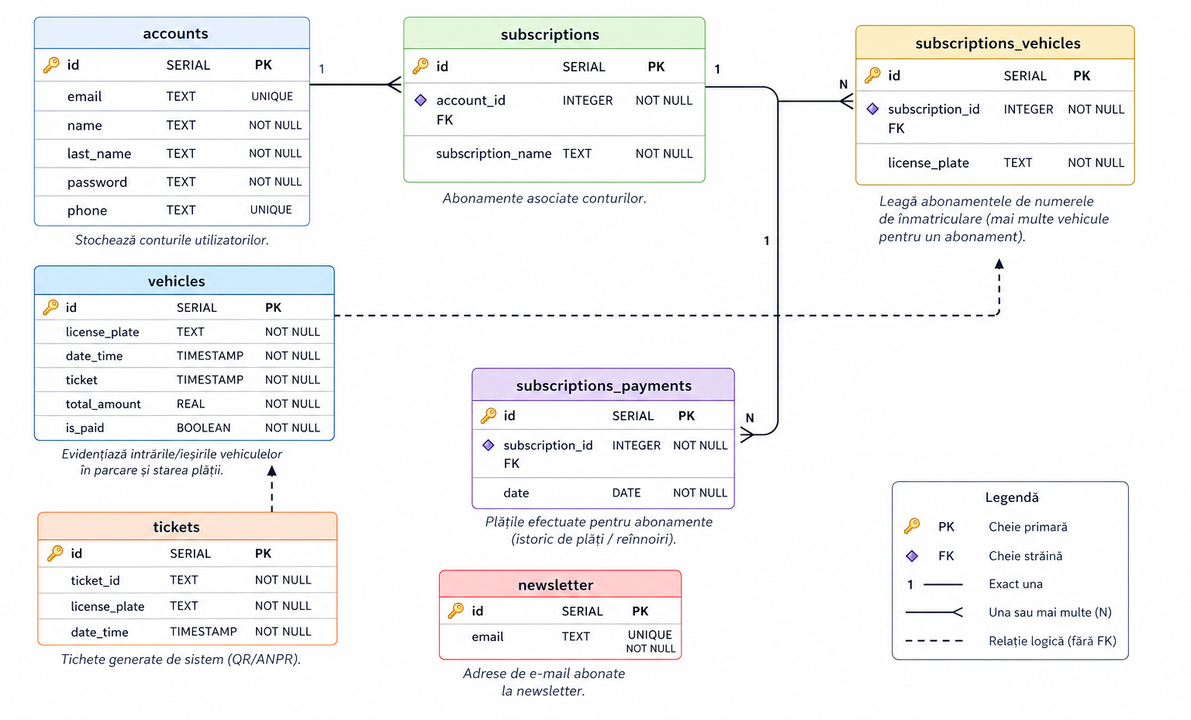
\includegraphics[width=0.75\textwidth]{images/bd.png}
    \caption{Diagrama bazei de date}
\end{figure}
\FloatBarrier

Tabelul \textit{Vehicles} este utilizat pentru memorarea accesărilor în parcare. Fiecare înregistrare conține numărul de înmatriculare, momentul asociat evenimentului, tichetul, suma totală și starea plății:

\[
    vehicle = \{license\_plate, date\_time, ticket, total\_amount, is\_paid\}
\]

Pentru conturile utilizatorilor, tabelul \textit{Accounts} memorează numele, prenumele, e-mailul, parola și numărul de telefon. E-mailul și telefonul sunt definite ca valori unice, deoarece acestea sunt utilizate pentru identificarea utilizatorului în procesul de autentificare și administrare a contului.

\[
    account = \{name, last\_name, email, password, phone\}
\]

Abonamentele sunt gestionate printr-o structură relațională. Tabelul \textit{Subscriptions} conține numele abonamentului și identificatorul contului asociat, iar tabelul \textit{Subscriptions\_Vehicles} leagă un abonament de unul sau mai multe numere de înmatriculare. Relațiile sunt definite cu chei străine, astfel, ștergerea unui cont sau a unui abonament determină eliminarea automată a datelor dependente.

\[
    account \rightarrow subscriptions \rightarrow subscriptions\_vehicles
\]

În momentul adăugării unui abonament, aplicația inserează mai întâi abonamentul în tabelul \textit{Subscriptions}, obține identificatorul generat și apoi creează o înregistrare în \textit{Subscriptions\_Payments}, folosind data curentă. În acest fel, sistemul păstrează o evidență a momentelor în care abonamentul a fost plătit sau reînnoit.

Tabelul \textit{Tickets} este folosit pentru stocarea tichetelor generate în urma procesării imaginilor sau a codurilor QR. Fiecare tichet conține un identificator, numărul de înmatriculare și data generării:

\[
    ticket = \{ticket\_id, license\_plate, date\_time\}
\]

Aceste informații pot fi returnate ulterior către aplicația desktop prin WebSocket, pentru afișare sau procesare operațională.

Operațiile asupra bazei de date sunt implementate folosind atât interogări simple, cât și interogări parametrizate. Pentru tratarea erorilor, fiecare operație verifică starea rezultatului returnat de PostgreSQL. Dacă interogarea eșuează, evenimentul este înregistrat prin sistemul de logare, memoria asociată rezultatului este eliberată, iar funcția returnează o valoare implicită sau oprește operația curentă. La închiderea aplicației, conexiunea la baza de date este eliberată.

Prin această organizare, sistemul de gestiune a bazei de date oferă o interfață unitară pentru restul aplicației. Serverul HTTP, serverul WebSocket și modulele de administrare nu lucrează direct cu PostgreSQL, ci folosesc metodele expuse de clasa \textit{DatabaseManager}. Astfel, logica de persistență este izolată într-o componentă separată, ceea ce face aplicația mai ușor de întreținut, extins și testat.

\section{Generarea și rularea serverului}

Pentru componenta de server, procesul de compilare și rulare a fost reproiectat pentru a asigura portabilitate, consistență între medii și ușurință în distribuire. Spre deosebire de abordarea inițială bazată exclusiv pe configurări locale CMake, versiunea actuală utilizează containere Docker, ceea ce permite rularea aplicației într-un mediu complet izolat și reproductibil.

Serverul este construit folosind un proces Docker în mai multe etape, împărțit în două faze principale:
\begin{itemize}
    \item etapa de compilare;
    \item etapa de execuție (imagine finală optimizată).
\end{itemize}

Această separare permite includerea tuturor dependențelor necesare compilării în prima etapă, fără a le transfera în imaginea finală, reducând astfel dimensiunea și suprafața de atac a containerului.

Pentru configurarea mediului de compilare, prima etapă pornește de la imaginea \texttt{ubuntu:22.04}, peste care sunt instalate toate dependențele necesare. Acestea includ:
\begin{itemize}
    \item compilatoare C/C++;
    \item biblioteci pentru baze de date;
    \item biblioteci pentru procesare JSON;
    \item biblioteci pentru criptografie și comunicații securizate;
    \item biblioteci pentru comunicații de rețea;
    \item biblioteci pentru procesare de imagini;
    \item biblioteci pentru integrarea serviciilor externe;
    \item utilitare generale necesare procesului de compilare.
\end{itemize}

Pentru a asigura consistența între medii, compilatorul utilizat este fixat la o versiune stabilă și compatibilă cu proiectul. Această alegere elimină diferențele între sisteme și reduce riscul apariției unor erori subtile de compilare.

Un aspect important al procesului este compilarea bibliotecii OpenCV direct din sursă, împreună cu modulele suplimentare. Aceasta este configurată astfel încât să includă doar componentele necesare aplicației, să dezactiveze exemplele și testele și să utilizeze standardul C++17. Această abordare oferă control complet asupra versiunii și configurației utilizate, evitând incompatibilitățile dintre distribuții.

În paralel, este utilizat un manager de pachete pentru C++ (\textit{vcpkg}) pentru instalarea și integrarea altor biblioteci externe, precum cele necesare comunicației prin WebSocket și cele pentru criptografie. Acest mecanism simplifică integrarea dependențelor și asigură o configurare coerentă a proiectului.

Codul sursă al serverului este copiat în container, iar procesul de compilare este realizat cu ajutorul CMake. Configurarea proiectului este realizată astfel încât să integreze automat bibliotecile instalate anterior, folosind mecanisme dedicate pentru gestionarea dependențelor. De asemenea, sunt definite explicit căile către anumite biblioteci externe pentru a asigura o legare corectă în timpul compilării.

După configurare, proiectul este compilat, rezultând un executabil complet al serverului.

Structura CMake a serverului reflectă o separare clară a responsabilităților:
\begin{itemize}
    \item definirea executabilului principal (\texttt{Server});
    \item includerea modulelor interne (HTTP, WebSocket, DatabaseManager);
    \item legarea bibliotecilor externe necesare;
    \item configurarea directoarelor de antet și a dependențelor.
\end{itemize}

Această organizare modulară permite extinderea facilă a serverului și integrarea de noi funcționalități fără modificări majore în infrastructura de compilare.

A doua etapă a procesului Docker pornește tot de la \texttt{ubuntu:22.04}, dar include doar dependențele necesare rulării aplicației:
\begin{itemize}
    \item biblioteci de execuție pentru C++;
    \item suport pentru baza de date PostgreSQL;
    \item module OpenCV necesare execuției;
    \item biblioteci pentru coduri QR;
    \item suport pentru comunicații securizate.
\end{itemize}

Executabilul compilat este transferat din etapa de compilare în imaginea finală, fără a include fișierele intermediare sau dependențele de compilare. În acest mod, imaginea rezultată este mai compactă și mai eficientă.

Pentru a evita problemele de legare dinamică, sunt configurate variabile de mediu astfel încât sistemul să poată localiza corect bibliotecile necesare la rulare. De asemenea, sunt create legături simbolice pentru anumite biblioteci, pentru a asigura compatibilitatea între diferite versiuni.

Pentru rularea containerului, serverul expune două porturi:
\begin{itemize}
    \item \textbf{8080} pentru comunicația HTTP;
    \item \textbf{9002} pentru comunicația WebSocket.
\end{itemize}

La pornirea containerului, este executat fișierul binar al serverului, care inițializează toate componentele sistemului: serverul HTTP, serverul WebSocket și conexiunea la baza de date. Astfel, aplicația devine imediat disponibilă pentru utilizare.

Utilizarea Docker pentru generarea și rularea serverului aduce multiple beneficii:
\begin{itemize}
    \item \textbf{portabilitate} – serverul poate rula identic pe orice sistem;
    \item \textbf{reproductibilitate} – mediul de compilare este complet determinist;
    \item \textbf{izolare} – dependențele nu interferează cu sistemul gazdă;
    \item \textbf{scalabilitate} – containerul poate fi integrat ușor în infrastructuri distribuite;
    \item \textbf{mentenanță simplificată} – actualizările se realizează prin reconstruirea imaginii.
\end{itemize}

În concluzie, procesul actual de generare și rulare al serverului combină flexibilitatea oferită de CMake cu avantajele containerizării Docker, rezultând un sistem modern, scalabil și ușor de distribuit.

\section{Prezentare generală a aplicației desktop}

Aplicația desktop reprezintă componenta locală a sistemului, utilizată pentru monitorizarea și administrarea fluxului de vehicule din parcare. Aceasta este dezvoltată în C++ și folosește framework-ul Qt pentru construirea interfeței grafice. Rolul principal al aplicației este de a permite operatorului să proceseze imagini cu vehicule, să urmărească intrările și ieșirile, să consulte tichetele generate și să vizualizeze statistici despre utilizarea parcării.

Interfața este construită în jurul ferestrei principale, reprezentată de clasa \texttt{MainWindow}. La inițializare, aceasta configurează toate elementele grafice, stabilește conexiunile dintre butoane și funcțiile aplicației și încarcă datele existente din sistem. Astfel, la pornire, aplicația reface starea curentă a parcării, afișând vehiculele deja înregistrate și tichetele disponibile.

\begin{figure}[htbp]
    \centering
    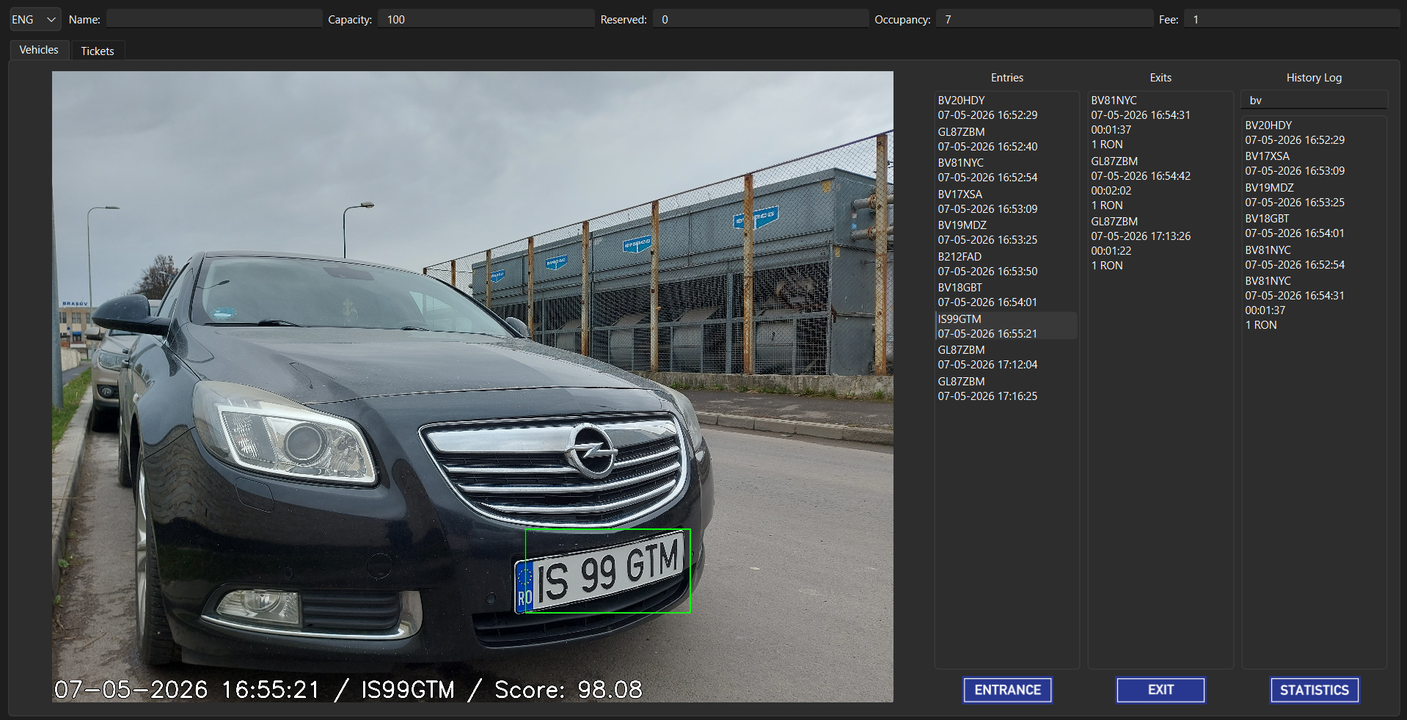
\includegraphics[width=0.8\textwidth]{images/gui.png}
    \caption{Interfața grafică principală}
\end{figure}
\FloatBarrier

Fereastra principală este împărțită în două zone importante. În partea superioară se află câmpurile de configurare generală ale parcării:
\begin{itemize}
    \item numele parcării;
    \item capacitatea totală;
    \item numărul de locuri rezervate;
    \item gradul de ocupare curent;
    \item taxa de parcare;
    \item limba interfeței.
\end{itemize}

Aceste câmpuri permit modificarea rapidă a parametrilor aplicației. Pentru valorile numerice, precum capacitatea, locurile rezervate și taxa, sunt folosiți validatori care acceptă doar numere întregi, prevenind introducerea unor date invalide.

Partea principală a interfeței este organizată în două file:
\begin{itemize}
    \item \textbf{Vehicles} -- pentru gestionarea vehiculelor;
    \item \textbf{Tickets} -- pentru gestionarea tichetelor.
\end{itemize}

Fila dedicată vehiculelor conține o zonă mare de afișare a imaginilor. În această zonă este afișată imaginea procesată a vehiculului, împreună cu rezultatele obținute în urma detecției numărului de înmatriculare.

În partea dreaptă a filei se află trei liste:
\begin{itemize}
    \item lista intrărilor;
    \item lista ieșirilor;
    \item istoricul vehiculelor.
\end{itemize}

Lista intrărilor reține vehiculele care au intrat în parcare, iar lista ieșirilor reține vehiculele care au părăsit parcarea. Istoricul permite căutarea și consultarea vehiculelor înregistrate anterior. Atunci când utilizatorul selectează un element dintr-o listă, aplicația încarcă imaginea asociată și o afișează în zona grafică principală.

Sub liste sunt amplasate butoanele de interacțiune. Butonul de intrare permite încărcarea unei imagini pentru un vehicul care intră în parcare, iar butonul de ieșire permite procesarea unei imagini pentru un vehicul care părăsește parcarea. Există și un buton pentru afișarea statisticilor, care deschide o fereastră separată dedicată analizei traficului din parcare.

Înainte de procesarea unei imagini, aplicația verifică starea parcării. Dacă se încearcă introducerea unui vehicul atunci când toate locurile sunt ocupate, utilizatorul primește un mesaj de avertizare. În mod similar, dacă se încearcă înregistrarea unei ieșiri atunci când nu există vehicule în parcare, operația este oprită.

După încărcarea unei imagini, aceasta este transmisă către componenta responsabilă cu gestionarea vehiculelor. Imaginea este procesată, iar aplicația obține informații precum numărul de înmatriculare, data și ora evenimentului și imaginea rezultată. În funcție de butonul apăsat, vehiculul este adăugat fie în lista de intrări, fie în lista de ieșiri.

În cazul în care vehiculul iese din parcare, aplicația verifică și starea plății. Dacă taxa nu a fost achitată, este afișată o fereastră modală de avertizare, reprezentată de clasa \texttt{UnpaidWindow}. Aceasta informează utilizatorul că plata nu a fost efectuată și oprește finalizarea operației de ieșire.

Dacă numărul de înmatriculare nu poate fi recunoscut, aplicația deschide o fereastră auxiliară, reprezentată de clasa \texttt{UploadQRWindow}. Prin aceasta, utilizatorul poate încărca imaginea codului QR asociat tichetului. Codul QR este apoi folosit pentru identificarea vehiculului și continuarea procesului de validare.

Fila dedicată tichetelor are o structură asemănătoare. În partea stângă se află o zonă grafică pentru afișarea imaginii tichetului, iar în partea dreaptă se află lista tichetelor active și un istoric al acestora. Selectarea unui tichet din listă determină încărcarea și afișarea imaginii asociate.

Aplicația primește tichete și prin mecanismul de comunicare în timp real cu serverul. Pentru acest lucru, în fereastra principală este configurat un callback care este apelat atunci când apare un tichet nou. Tichetul este procesat, textul de afișare este generat, iar elementul nou este adăugat automat în lista de tichete.

\begin{sloppypar}
O funcționalitate importantă a aplicației este afișarea statisticilor. Fereastra \texttt{StatisticsWindow} prezintă datele sub forma unui tabel cu zilele săptămânii și orele zilei. Utilizatorul poate alege între trei tipuri de statistici:
\end{sloppypar}
\begin{itemize}
    \item gradul de ocupare;
    \item numărul de intrări;
    \item numărul de ieșiri.
\end{itemize}

Valorile sunt normalizate și reprezentate vizual prin intensitatea culorii celulelor din tabel. Astfel, perioadele cu activitate mai mare pot fi identificate rapid, fără a analiza manual fiecare valoare numerică.

Interfața permite și schimbarea limbii. Utilizatorul poate alege între engleză și română, iar aplicația încarcă fișierele de traducere corespunzătoare. După schimbarea limbii, interfața este reconstruită pentru ca textele afișate să fie actualizate.

Prin această organizare, aplicația desktop oferă o interfață completă pentru operarea locală a parcării. Utilizatorul poate procesa intrări și ieșiri, verifica tichete, urmări istoricul vehiculelor, consulta statistici și modifica parametrii principali ai parcării. Separarea funcționalităților în ferestre și file distincte contribuie la claritatea interfeței și la ușurința utilizării în scenarii reale de monitorizare.

\section{Generarea și configurarea aplicației desktop}

Pentru aplicația desktop, procesul de generare și configurare este realizat cu ajutorul CMake. Proiectul este organizat modular, fiecare componentă importantă având propriul fișier de configurare. Această abordare permite separarea responsabilităților și simplifică atât procesul de compilare, cât și întreținerea aplicației.

Configurația principală a aplicației stabilește versiunea minimă de CMake, numele proiectului, standardul C++ utilizat și directorul în care vor fi generate fișierele executabile. Proiectul folosește standardul C++17, deoarece acesta oferă funcționalități moderne necesare implementării componentelor aplicației.

De asemenea, configurația globală setează proiectul \texttt{Application} ca proiect de pornire în Visual Studio. Astfel, la deschiderea soluției, mediul de dezvoltare poate porni direct aplicația desktop principală, fără configurări suplimentare din partea dezvoltatorului.

Structura aplicației este împărțită în mai multe module:
\begin{itemize}
    \item \textbf{Logger} - pentru înregistrarea mesajelor și erorilor;
    \item \textbf{LicensePlateDetection} - pentru detecția și recunoașterea numerelor de înmatriculare;
    \item \textbf{QRCodeDetection} - pentru detecția și decodarea codurilor QR;
    \item \textbf{WebSocketClient} - pentru comunicarea în timp real cu serverul;
    \item \textbf{VehicleManager} - pentru coordonarea operațiilor legate de vehicule;
    \item \textbf{Interface} - pentru interfața grafică;
    \item \textbf{Application} - pentru executabilul final al aplicației desktop.
\end{itemize}

Modulul \texttt{Logger} este configurat ca bibliotecă dinamică. Acesta colectează automat fișierele sursă și antet din directorul propriu și expune funcționalitățile necesare celorlalte componente ale aplicației. Separarea acestui modul este utilă deoarece sistemul de logare poate fi folosit independent de logica de interfață, procesare imagini sau comunicație.

Modulul \texttt{LicensePlateDetection} este, de asemenea, construit ca bibliotecă dinamică. Acesta integrează bibliotecile OpenCV și Tesseract, necesare pentru procesarea imaginilor și recunoașterea optică a caracterelor. Prin această configurare, funcționalitățile de detecție a numerelor de înmatriculare sunt izolate într-o componentă separată, care poate fi dezvoltată și testată independent.

Modulul \texttt{QRCodeDetection} este responsabil pentru detecția și decodarea codurilor QR. Acesta este construit ca bibliotecă dinamică și folosește OpenCV pentru procesarea imaginilor, respectiv ZXing pentru decodarea conținutului codurilor QR. Astfel, aplicația poate trata separat fluxul de procesare a codurilor QR față de cel al numerelor de înmatriculare.

Modulul \texttt{WebSocketClient} este configurat ca bibliotecă dinamică și include dependențele necesare comunicației în timp real. Acesta utilizează Boost.Beast și Boost.Asio pentru conexiunea WebSocket, iar nlohmann::json pentru construirea și interpretarea mesajelor în format JSON. În plus, modulul depinde de \texttt{Logger}, pentru a putea înregistra erorile sau evenimentele apărute în timpul comunicației cu serverul.

Modulul \texttt{VehicleManager} are rol de componentă intermediară între interfața grafică, modulele de procesare și clientul WebSocket. Acesta este construit ca bibliotecă dinamică și depinde de \texttt{QRCodeDetection}, \texttt{LicensePlateDetection} și \texttt{WebSocketClient}. Prin această organizare, logica legată de vehicule este centralizată, iar interfața grafică nu trebuie să comunice direct cu fiecare modul tehnic în parte.

Modulul \texttt{Interface} este construit ca bibliotecă statică și reprezintă componenta responsabilă pentru interfața grafică a aplicației. Pentru integrarea cu Qt, este activată procesarea automată a fișierelor care folosesc mecanismul de semnale și sloturi. Modulul folosește componentele Qt pentru ferestre, elemente grafice și logica de interfață, iar dependența principală este \texttt{VehicleManager}, prin care sunt accesate funcționalitățile aplicației.

Executabilul final este definit în modulul \texttt{Application}. Acesta include fișierele sursă principale și este generat ca aplicație Windows, cu numele final \texttt{ParkingLotsSecurityCamera}. Executabilul depinde de modulul \texttt{Interface}, iar prin acesta are acces indirect la toate celelalte componente: gestionarea vehiculelor, comunicarea WebSocket, detecția codurilor QR, recunoașterea numerelor de înmatriculare și logarea evenimentelor.

Pentru distribuirea aplicației, configurația CMake definește și un director de livrare, denumit \texttt{deliverypack}. În acest director sunt instalate executabilul final, bibliotecile dinamice necesare rulării, extensiile Qt, fișierele Tesseract, biblioteca pentru coduri QR și resursele aplicației.

Resursele copiate în pachetul final includ imagini utilizate de interfață, șablonul pentru litera \texttt{I}, fișiere text pentru vehicule și abonamente, precum și fișierele de traducere ale aplicației. De asemenea, sunt create automat directoare pentru stocarea locală a imaginilor vehiculelor și tichetelor.

Prin această configurare, aplicația desktop este generată ca un ansamblu modular, în care fiecare parte are un rol bine definit. CMake coordonează ordinea de compilare, legarea bibliotecilor și pregătirea pachetului final de livrare. Astfel, proiectul poate fi compilat, rulat și distribuit într-un mod organizat, iar adăugarea unor funcționalități noi poate fi realizată fără modificarea majoră a întregii structuri.

\section{Prezentare generală a website-ului}

Aplicația web reprezintă interfața destinată utilizatorilor și administratorilor sistemului, oferind acces la funcționalitățile principale ale parcării prin intermediul unui browser. Aceasta este dezvoltată folosind framework-ul Angular și este organizată sub forma unei aplicații de tip Single Page Application (SPA), în care navigarea între pagini se realizează fără reîncărcarea completă a conținutului.

Structura aplicației este bazată pe un sistem de rutare, fiecare funcționalitate fiind asociată unei pagini (componentă) distincte. Interfața este împărțită în mai multe pagini principale, fiecare corespunzând unui set de funcționalități specifice. Aceste pagini sunt implementate sub formă de componente Angular și sunt organizate în directoare separate în cadrul proiectului.

Navigarea între pagini este realizată prin intermediul unui sistem de tab-uri sau link-uri din bara de navigare, fiecare tab având un rol bine definit în cadrul aplicației.

Prima interacțiune a utilizatorului cu aplicația este realizată prin pagina de autentificare. Aceasta include următoarele funcționalități:
\begin{itemize}
    \item autentificarea utilizatorilor existenți;
    \item crearea unui cont nou;
    \item validarea datelor introduse (email, parolă);
    \item integrarea mecanismului Google reCAPTCHA pentru prevenirea abuzurilor.
\end{itemize}

În cazul creării unui cont, utilizatorul este redirecționat către un proces de validare, în care trebuie să introducă un cod primit prin email sau SMS.

\begin{figure}[htbp]
    \centering
    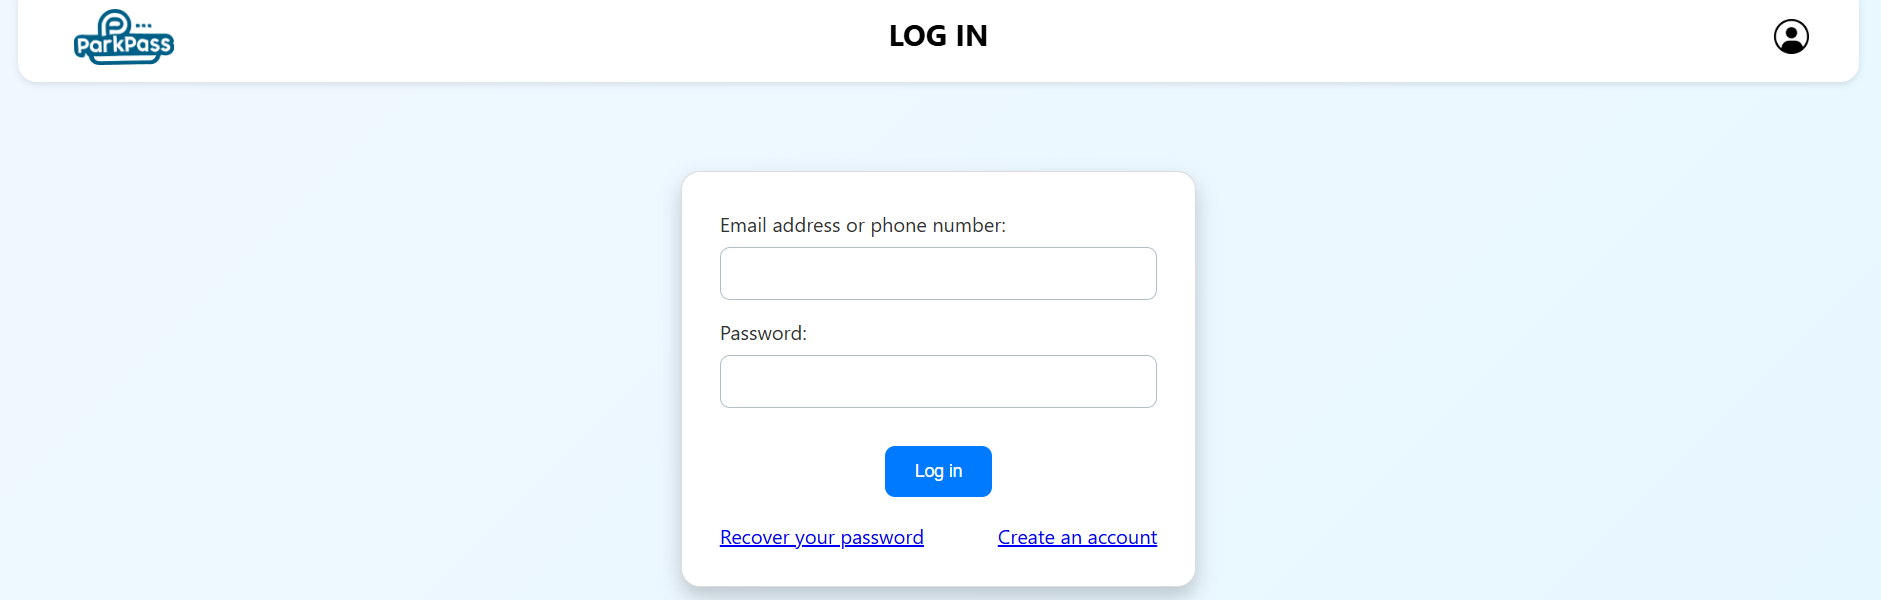
\includegraphics[width=0.75\textwidth]{images/web1.png}
    \caption{Pagina de autentificare a aplicației web}
\end{figure}
\FloatBarrier

După autentificare, utilizatorul este redirecționat către pagina principală, care oferă o vedere de ansamblu asupra contului. Această pagină poate include:
\begin{itemize}
    \item informații despre utilizator;
    \item acces rapid către celelalte secțiuni ale aplicației;
    \item statusul abonamentelor și al vehiculelor asociate.
\end{itemize}

Dashboard-ul funcționează ca punct central de navigare în aplicație.

\begin{figure}[htbp]
    \centering
    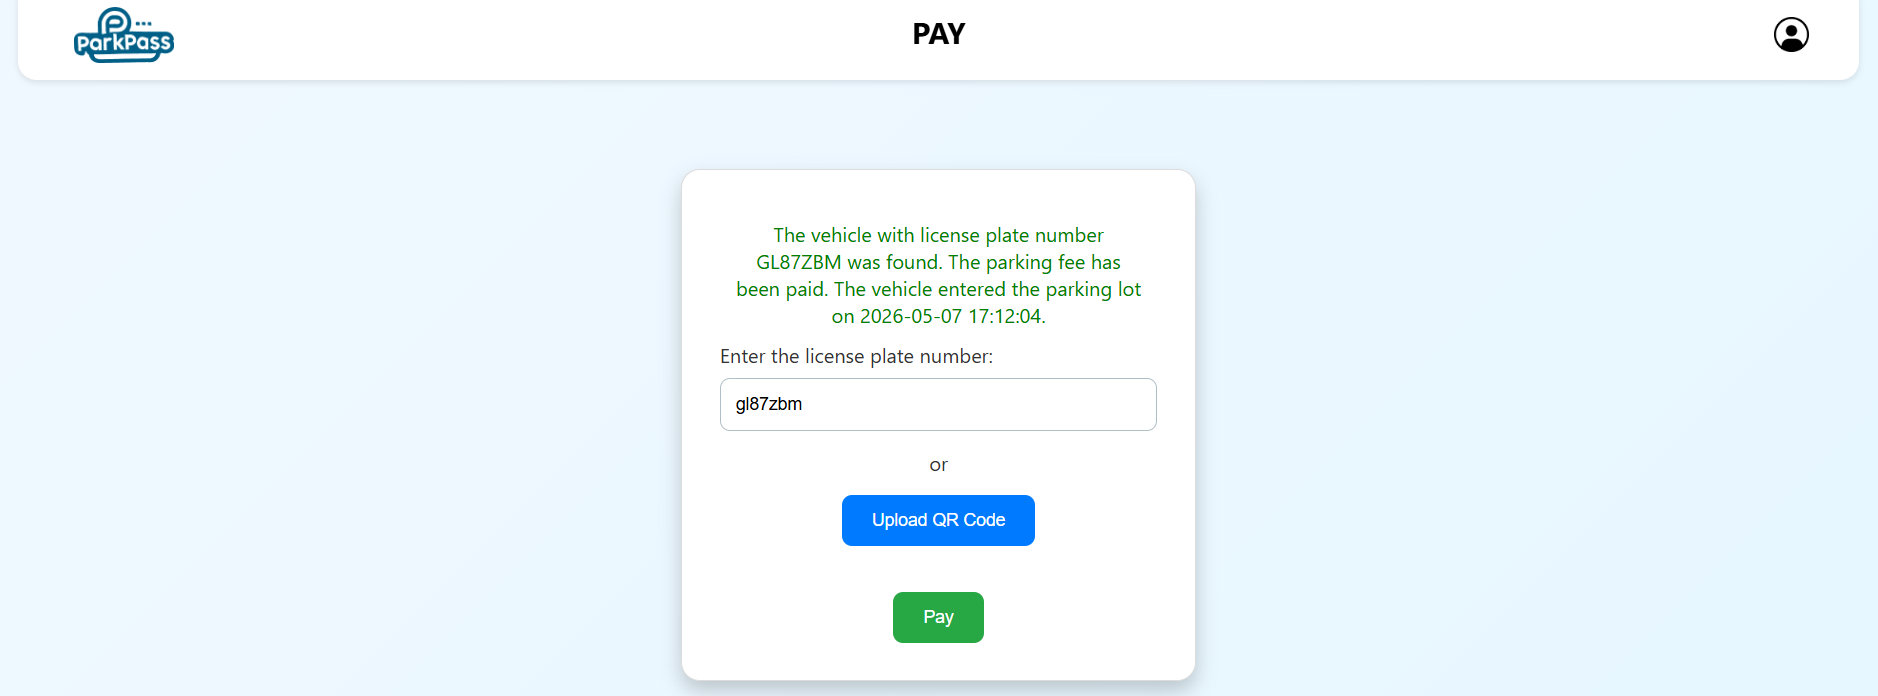
\includegraphics[width=0.75\textwidth]{images/web4.png}
        \caption{Pagina principală a aplicației web}
\end{figure}
\FloatBarrier

Secțiunea dedicată profilului utilizatorului permite vizualizarea și modificarea datelor personale:
\begin{itemize}
    \item nume și prenume;
    \item adresă de email;
    \item număr de telefon;
    \item schimbarea parolei.
\end{itemize}

Această pagină comunică direct cu serverul pentru actualizarea informațiilor și validarea modificărilor.

\begin{figure}[htbp]
    \centering
    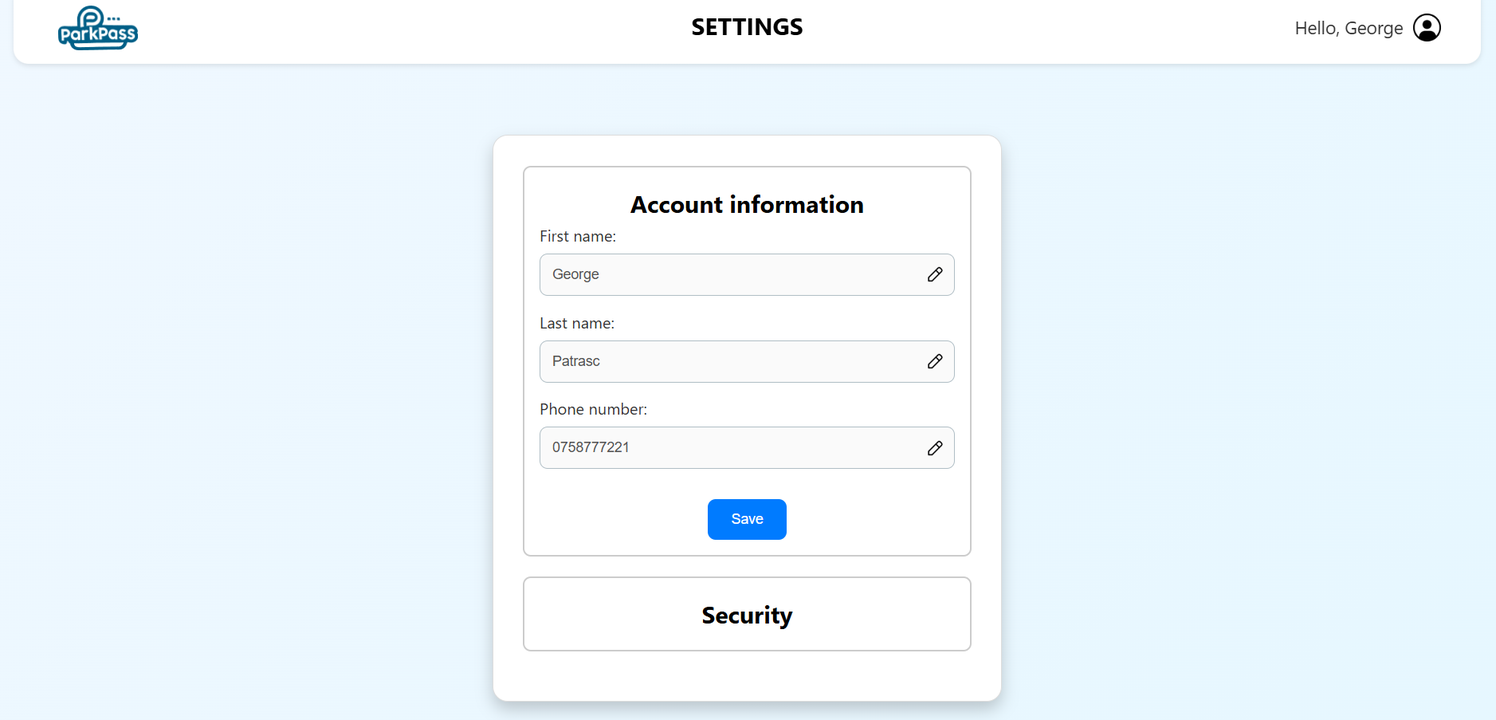
\includegraphics[width=0.75\textwidth]{images/web3.png}
    \caption{Pagina de administrare a profilului utilizatorului}
\end{figure}
\FloatBarrier

Unul dintre cele mai importante module ale aplicației este cel dedicat abonamentelor. În această secțiune, utilizatorul poate:
\begin{itemize}
    \item vizualiza lista abonamentelor existente;
    \item crea un abonament nou;
    \item șterge abonamente;
    \item consulta vehiculele asociate fiecărui abonament;
    \item verifica istoricul plăților.
\end{itemize}

Interfața este organizată sub formă de liste sau tabele, fiecare abonament fiind reprezentat printr-un element care poate fi selectat pentru a afișa detalii suplimentare.

\begin{figure}[htbp]
    \centering
    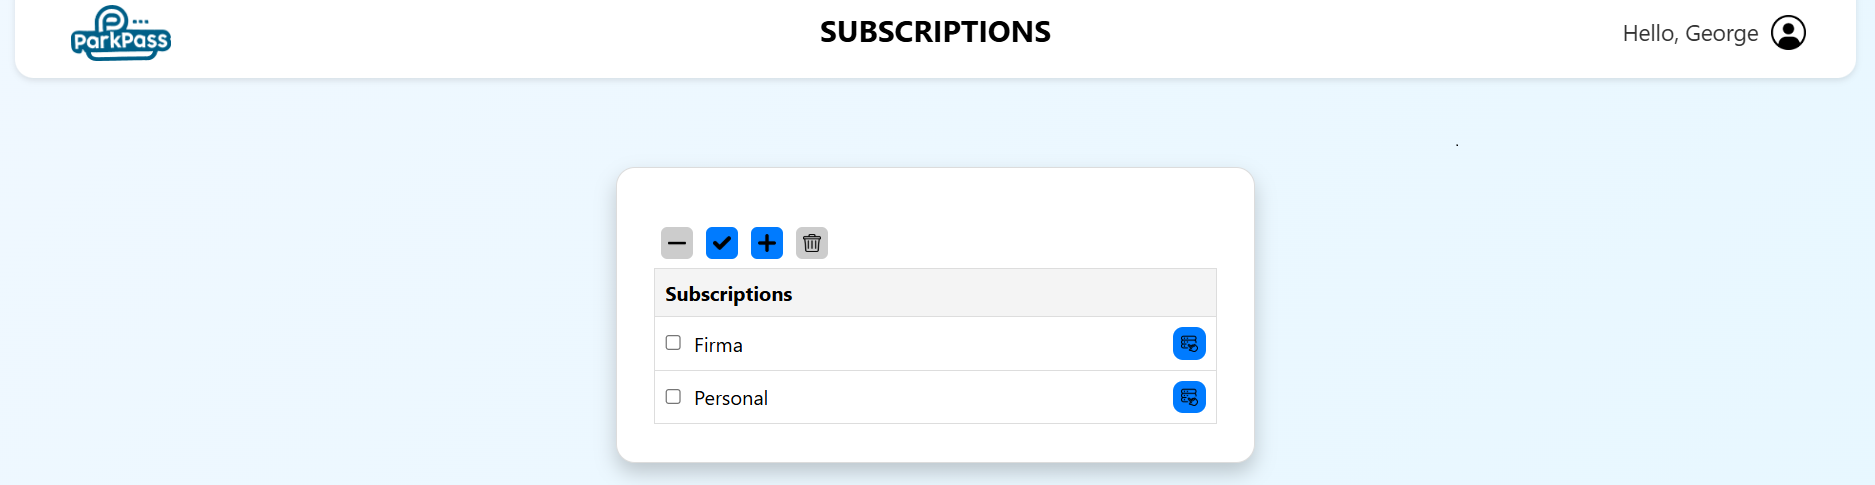
\includegraphics[width=0.75\textwidth]{images/web2.png}
    \caption{Pagina de gestionare a abonamentelor}
\end{figure}
\FloatBarrier

Această secțiune permite utilizatorului să administreze vehiculele asociate abonamentelor:
\begin{itemize}
    \item adăugarea unui nou vehicul (număr de înmatriculare);
    \item eliminarea unui vehicul existent;
    \item vizualizarea istoricului accesărilor;
    \item afișarea timpului petrecut în parcare și a costurilor asociate.
\end{itemize}

Numerele de înmatriculare sunt normalizate automat pentru a asigura consistența datelor.

Aplicația oferă o secțiune dedicată istoricului, unde utilizatorul poate consulta:
\begin{itemize}
    \item intrările și ieșirile din parcare;
    \item durata fiecărei sesiuni;
    \item costurile calculate;
    \item starea plății.
\end{itemize}

Datele sunt afișate într-un format tabelar, fiind preluate din baza de date prin intermediul serverului.

\begin{figure}[htbp]
    \centering
    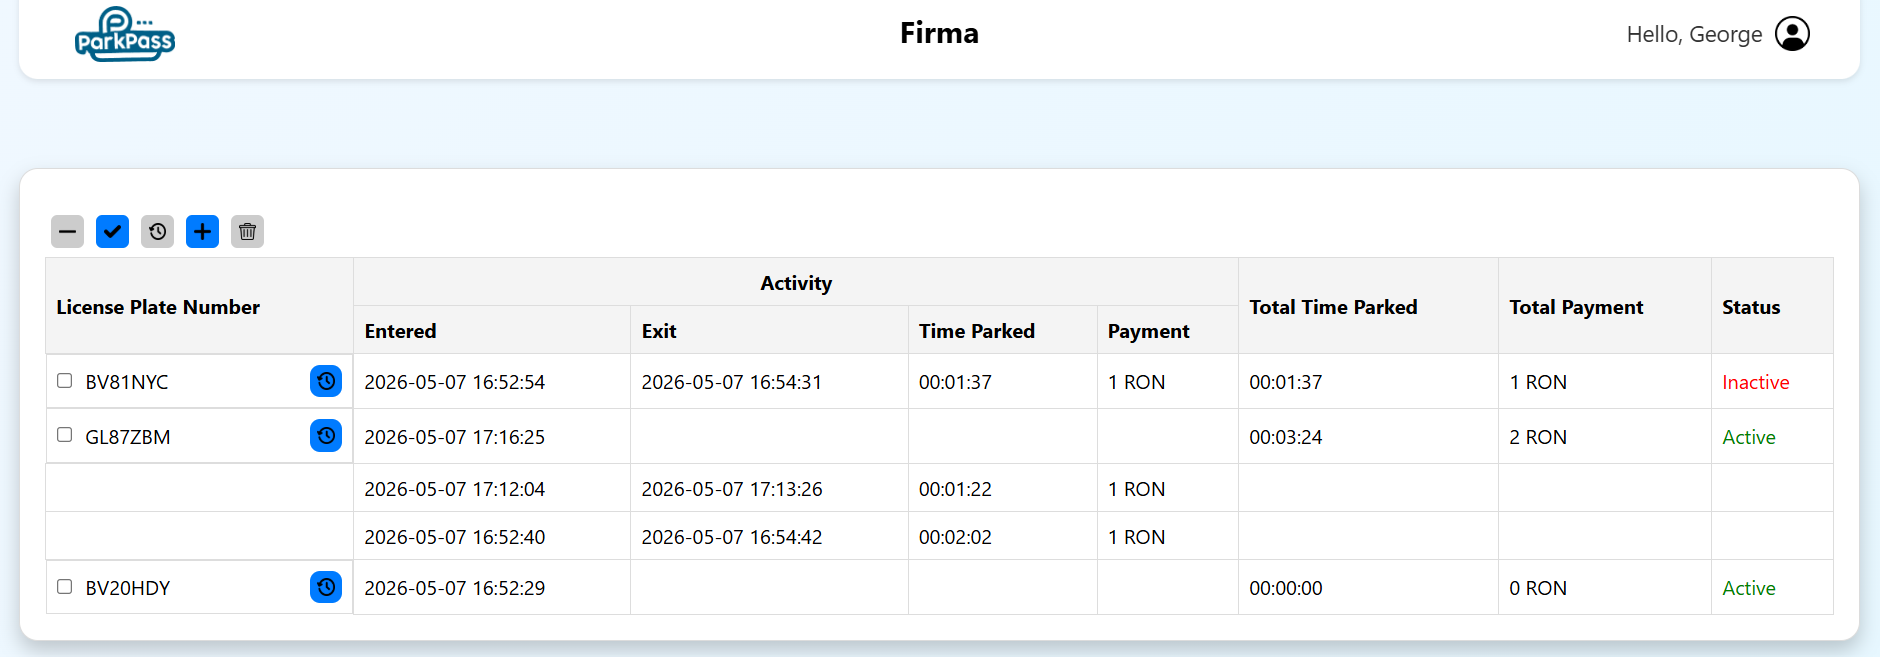
\includegraphics[width=0.75\textwidth]{images/web5.png}
    \caption{Pagina de gestionare a vehiculelor și a istoricului accesărilor}
\end{figure}
\FloatBarrier

Aplicația include și o secțiune de contact, prin care utilizatorii pot:
\begin{itemize}
    \item trimite mesaje către administrator;
    \item primi răspunsuri automate;
    \item gestiona abonarea la newsletter.
\end{itemize}

Această componentă facilitează comunicarea directă între utilizatori și sistem.

\begin{figure}[htbp]
    \centering
    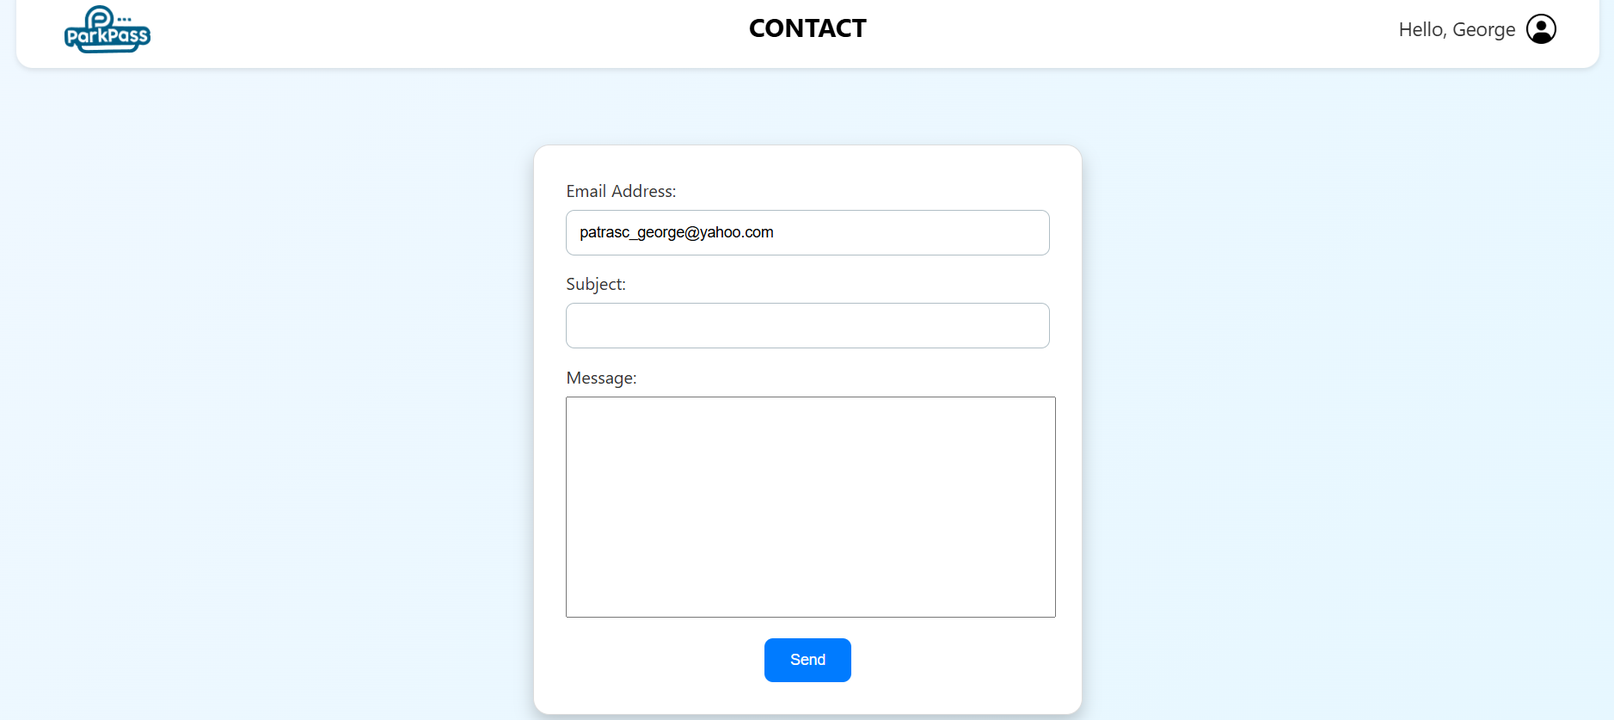
\includegraphics[width=0.75\textwidth]{images/web6.png}
    \caption{Pagina de contact a aplicației web}
\end{figure}
\FloatBarrier

Pentru utilizatorii cu rol de administrator, aplicația oferă o secțiune suplimentară care permite:
\begin{itemize}
    \item vizualizarea tuturor utilizatorilor;
    \item gestionarea conturilor;
    \item monitorizarea activității din sistem.
\end{itemize}

Accesul la această secțiune este restricționat și validat prin mecanisme separate de autentificare.

\begin{figure}[htbp]
    \centering
    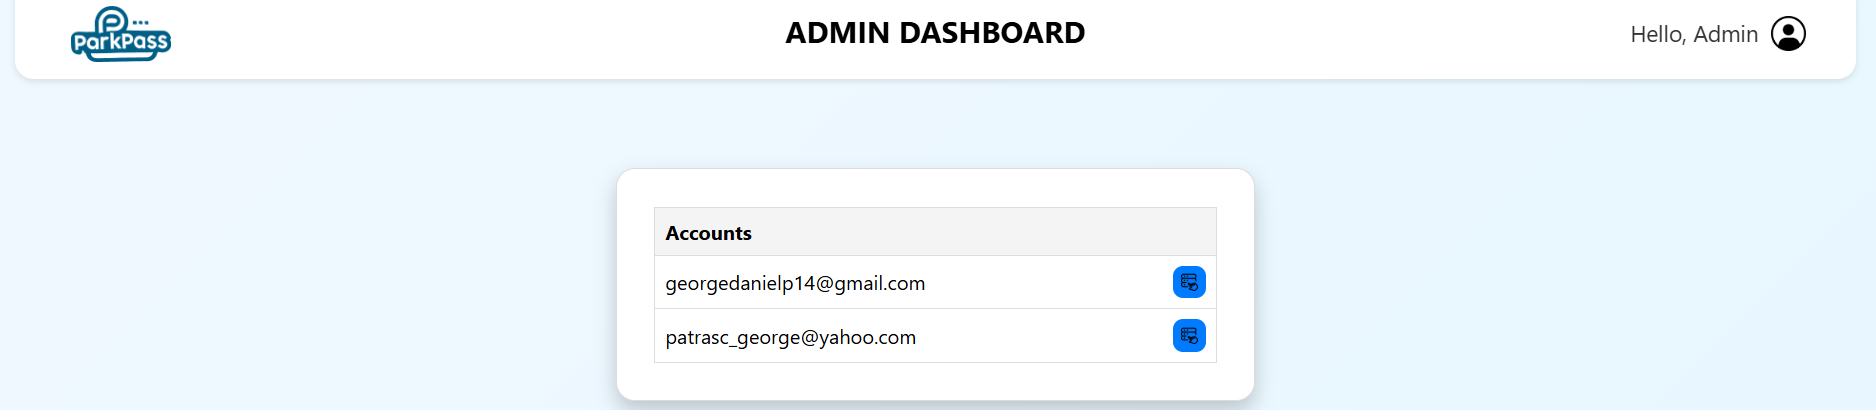
\includegraphics[width=0.75\textwidth]{images/web7.png}
    \caption{Pagina de administrare a sistemului}
\end{figure}
\FloatBarrier

Toate paginile aplicației comunică cu serverul prin cereri HTTP. Datele sunt transmise și primite în format JSON, iar fiecare acțiune din interfață corespunde unui endpoint specific din server. Pentru securitate, fiecare cerere include o cheie de acces, iar răspunsurile sunt validate înainte de a fi afișate utilizatorului.

În cadrul proiectului Angular, fiecare funcționalitate este implementată într-un director separat, care conține:
\begin{itemize}
    \item fișierul de logică (\texttt{.ts});
    \item template-ul HTML;
    \item stilurile asociate (\texttt{.css} sau \texttt{.scss}).
\end{itemize}

Această structură modulară permite dezvoltarea independentă a fiecărei componente și facilitează extinderea aplicației.

Aplicația web oferă o interfață completă pentru gestionarea interacțiunii utilizatorilor cu sistemul de parcare. Prin organizarea în pagini și module distincte, aceasta permite administrarea conturilor, abonamentelor și vehiculelor, precum și consultarea istoricului și comunicarea cu sistemul. Integrarea cu serverul și utilizarea unei arhitecturi modulare contribuie la scalabilitatea și flexibilitatea aplicației.

\section{Deployment-ul website-ului}

Pentru aplicația web, procesul de generare și publicare este realizat prin Docker. Această abordare permite construirea website-ului într-un mediu controlat și rularea lui într-un container separat, fără ca sistemul gazdă să aibă nevoie de instalarea manuală a Node.js, Angular CLI sau Nginx.

Procesul este împărțit în două etape principale:
\begin{itemize}
    \item etapa de construire a aplicației Angular;
    \item etapa de servire a fișierelor statice prin Nginx.
\end{itemize}

Prima etapă pornește de la o imagine Node.js, folosită pentru instalarea dependențelor și compilarea aplicației Angular. În această etapă sunt copiate fișierele proiectului, inclusiv fișierele de configurare ale pachetelor, codul sursă și scripturile auxiliare.

Aplicația web este definită ca proiect Angular și sunt stabilite directorul sursă, fișierul principal al aplicației, fișierul HTML de intrare, stilurile globale și resursele statice.

Configurarea Angular include și o variantă de producție. Aceasta activează optimizările necesare pentru publicare, precum generarea numelor de fișiere cu identificatori unici și verificarea dimensiunii pachetelor generate. Astfel, website-ul rezultat este mai potrivit pentru rularea într-un mediu real, unde sunt importante atât performanța, cât și livrarea eficientă a fișierelor către utilizator.

Proiectul folosește Angular, modulele necesare pentru formulare, rutare, animații și randare în browser, precum și biblioteca \texttt{ng-recaptcha}, utilizată pentru integrarea mecanismului Google reCAPTCHA. În același fișier sunt definite și comenzile de dezvoltare, testare și construire a aplicației.

Înainte de compilarea propriu-zisă, este executat un script auxiliar care generează fișiere în directoarele componentei Angular. Aceste fișiere conțin valori de configurare sub formă de șabloane, precum adresa serverului și parola folosită în anumite cereri. Valorile nu sunt fixate direct în codul sursă, ci sunt lăsate ca marcaje ce vor fi înlocuite ulterior la pornirea containerului.

Această strategie este utilă deoarece aceeași imagine Docker poate fi folosită în mai multe medii. De exemplu, aplicația poate fi rulată local, pe un server de test sau într-un mediu de producție, schimbând doar variabilele de mediu transmise containerului, fără a reconstrui codul Angular pentru fiecare caz.

După generarea fișierelor de mediu, sunt instalate dependențele proiectului. Instalarea folosește opțiuni care permit rezolvarea dependențelor chiar și în situațiile în care unele pachete au cerințe mai vechi sau mai stricte între versiuni. Ulterior, aplicația este compilată folosind configurația de producție, rezultând fișiere statice HTML, CSS și JavaScript.

A doua etapă pornește de la o imagine Nginx bazată pe Alpine Linux. Aceasta este mai redusă ca dimensiune și este potrivită pentru servirea fișierelor statice generate anterior. În imaginea finală nu mai sunt păstrate dependențele Node.js sau fișierele intermediare de compilare, ci doar rezultatul final al aplicației Angular.

Fișierele generate în etapa de construire sunt copiate în directorul standard folosit de Nginx pentru conținut web. Astfel, la pornirea containerului, Nginx poate livra direct aplicația web către browserul utilizatorului.

Pentru configurarea valorilor dependente de mediu, în imaginea finală este inclus și scriptul care parcurge fișierele generate ale aplicației și înlocuiește marcajele de tip șablon cu valorile reale primite prin variabile de mediu. În acest fel, adresa serverului poate fi stabilită la rulare, fără modificarea sau recompilarea aplicației.

Containerul expune portul 80, folosit pentru accesarea website-ului prin HTTP. La pornire, se execută mai întâi scriptul de înlocuire a variabilelor de mediu, apoi este pornit Nginx în prim-plan. Această ordine este importantă deoarece aplicația trebuie să aibă valorile corecte de configurare înainte de a fi servită utilizatorilor.

Prin această configurare, website-ul este separat clar în două faze: construirea aplicației Angular și servirea rezultatului final. Prima fază are nevoie de Node.js și de toate instrumentele de compilare, iar a doua fază are nevoie doar de Nginx și de fișierele statice generate.

Utilizarea Docker pentru aplicația web aduce mai multe avantaje:
\begin{itemize}
    \item \textbf{portabilitate} -- website-ul poate fi rulat identic pe sisteme diferite;
    \item \textbf{separarea mediilor} -- etapa de construire este separată de etapa de rulare;
    \item \textbf{configurare flexibilă} -- valorile precum adresa serverului pot fi schimbate prin variabile de mediu;
    \item \textbf{imagine finală redusă} -- în producție sunt păstrate doar fișierele necesare servirii website-ului;
    \item \textbf{distribuire simplificată} -- aplicația poate fi publicată prin rularea containerului Nginx.
\end{itemize}

În concluzie, aplicația web este generată ca proiect Angular și publicată printr-un container Nginx. Docker asigură un proces reproductibil de construire, iar mecanismul de înlocuire a variabilelor de mediu permite adaptarea website-ului la diferite medii fără modificarea codului sursă.
